%%%%%%%%%%%%%%%%%%%%%%%%%%%%%%%%%%%%%%%%%%%%%%%%%
%%%%%%%%%%%%%%%%%%%%%%%%%%%%%%%%%%%%%%%%%%%%%%%%%%%
% !TeX program = lualatex
\documentclass[a4paper,12pt,oneside,final]{mwrep}
\usepackage{polyglossia}
\setdefaultlanguage{polish}
\setmainfont{Iwona}
%%%%%%%%%%%%%%%%%%%%%%%%%%%%%%%%%%%%%%%%%%%%%%%%%%%%%%%%%
% Source: http://en.wikibooks.org/wiki/LaTeX/Hyperlinks %
%%%%%%%%%%%%%%%%%%%%%%%%%%%%%%%%%%%%%%%%%%%%%%%%%%%%%%%%%
\usepackage{graphicx}
\usepackage{booktabs}
\usepackage[bookmarks]{hyperref}
\usepackage{tcolorbox}
\usepackage{url}
\usepackage{lscape}
\usepackage{array}
\usepackage{chngpage}
\usepackage{caption}
\DeclareCaptionFont{white}{\color{white}}
\DeclareCaptionFormat{listing}{\colorbox{gray}{\parbox{\textwidth}{#1#2#3}}}
\captionsetup[lstlisting]{format=listing,labelfont=white,textfont=white}
\usepackage{subcaption} 
\captionsetup{compatibility=false}
\usepackage{listings}
\usepackage{underscore}
\usepackage{longtable}
\usepackage[toc,page]{appendix}
\usepackage{epstopdf}
\usepackage{pdflscape}
\usepackage{xcolor}
\lstset{basicstyle=\footnotesize\ttfamily,breaklines=true}
\lstset{framextopmargin=50pt,commentstyle=\itshape\color{purple!40!black}}
\lstset{
	escapeinside={\%*}{*)}
}
\lstset{extendedchars=true,inputencoding=utf8x,literate=%
	{ą}{{\k{a}}}1
	{Ą}{{\k{A}}}1
	{ę}{{\k{e}}}1
	{Ę}{{\k{E}}}1
	{ó}{{\'o}}1
	{Ó}{{\'O}}1
	{ś}{{\'s}}1
	{Ś}{{\'S}}1
	{ł}{{\l{}}}1
	{Ł}{{\L{}}}1
	{ż}{{\.z}}1
	{Ż}{{\.Z}}1
	{ź}{{\'z}}1
	{Ź}{{\'Z}}1
	{ć}{{\'c}}1
	{Ć}{{\'C}}1
	{ń}{{\'n}}1
	{Ń}{{\'N}}1
}

\usepackage{filecontents}
\begin{filecontents*}{Bibliografy.bib}
	@book{Corti:2014:PC:2616182,
		author = {Corti, Paolo and Mather, Stephen Vincent and Kraft, Thomas J and Park, Borie},
		isbn = {1849518661, 9781849518666},
		publisher = {Packt Publishing},
		title = {{PostGIS Cookbook}},
		year = {2014}
	}
	@book{Obe:2011:PA:2018871,
		address = {Greenwich, CT, USA},
		author = {Obe, Regina and Hsu, Leo},
		isbn = {1935182269, 9781935182269},
		publisher = {Manning Publications Co.},
		title = {{PostGIS in Action}},
		year = {2011}
	}
	@book{Iwanczak2013,
		address = {Gliwice},
		author = {Iwa{\'{n}}czak, Bart{\l}omiej},
		publisher = {Helion},
		title = {{Quantium GIS. Tworzenie i analiza map}},
		year = {2013}
	}
	
\end{filecontents*}
\usepackage[numbers]{natbib}
\bibliographystyle{plplain}


% Book's title and subtitle
\title{\Huge \textbf{Schematy GIS Kultura}  \\ \huge Zarządzanie bazami i danymi OpenStreetMap. }
% Author
\author{\textsc{dr Mariusz Piotrowski}}
\date{\today\\wersja robocza}

\begin{document}

%\frontmatter
\maketitle



%%%%%%%%%%%%%%%%%%%%%%%%%%%%%%%%%%%%%%%%%%%%%%%%%%%%%%%%%%%%%%%%%%%%%%%%
% Auto-generated table of contents, list of figures and list of tables %
%%%%%%%%%%%%%%%%%%%%%%%%%%%%%%%%%%%%%%%%%%%%%%%%%%%%%%%%%%%%%%%%%%%%%%%%
\tableofcontents
\listoffigures
\lstlistoflistings
%\mainmatter

%%%%%%%%%%%
% Preface %
%%%%%%%%%%%
\chapter*{Informacje wstępne}
Dokument ma charakter technicznego wprowadzenia w projekt GIS Kultura. Prezentowane są narzędzia i sposoby porządkowania zgromadzonych danych.\par
Dzięki zaprezentowanym metodom i zmodyfikowanym plikom znajdującym się w Aneksie, możliwa jest replikacja systemu we własnym środowisku. Komendy skryptów testowane były w systemach Linux i macOS. Niniejszy plik zawiera kody i komendy, ale zdecydowanie odradzam używanie ich bez zrozumienia sensu działania. Dodatkowo w czasie kopiowania z pliku pdf mogą pojawić się błędy w spacjach i końcach linii.
 Dokument prezentuje jedynie fragment pracy na zgromadzonych bazach danych.\par
\paragraph{O badaniach OSM.} 
W przyjętej perspektywie naukowej dane OSM stanowią dane, które używa się w celach poznawczych i opisowych. Są traktowane jako źródło wiedzy o rzeczywistości. Przyjąć należy jednak pewną dozę sceptycyzmu dotyczącego samego źródła informacji. OpenStreetMap jest projektem społecznościowym, w którym standardy powstały w drodze konsensusu, który nie zawsze respektuje ustalenia innych projektów, czy zwyczajów klasyfikacji obiektów.\par
Osobne klasy problemów badawczych, które dotyczą OSM można określić jako:
\begin{itemize}
	\item badania nad jakością danych (obszar refleksji geografów i kartografów);
	\item badania nad czynnikami społecznymi, które wpływają na kontrybucję;
	\item badania dotyczące społecznych praktyk uczestników projektu OSM;
	\item badania nad procesami klasyfikowania i typologizacji obiektów;
	
\end{itemize}


\begin{tcolorbox}
Najważniejszym wyzwaniem w projekcie jest uwzględnienie w bazie znacznika czasu, który pozwoli na wykonywanie analiz szeregów czasowych. Wymaga to stworzenia infrastruktury aktualizacji i przechowywania danych.
Np. Przyrostu określonych typów obiektów.
\end{tcolorbox}

\chapter{Specyfika projektu OSM}
\section{Architektura systemu OpenStreetMap.}

\begin{landscape}
	\begin{figure}[htp]
		\caption{Pełne dane OSM.}
	\centering
	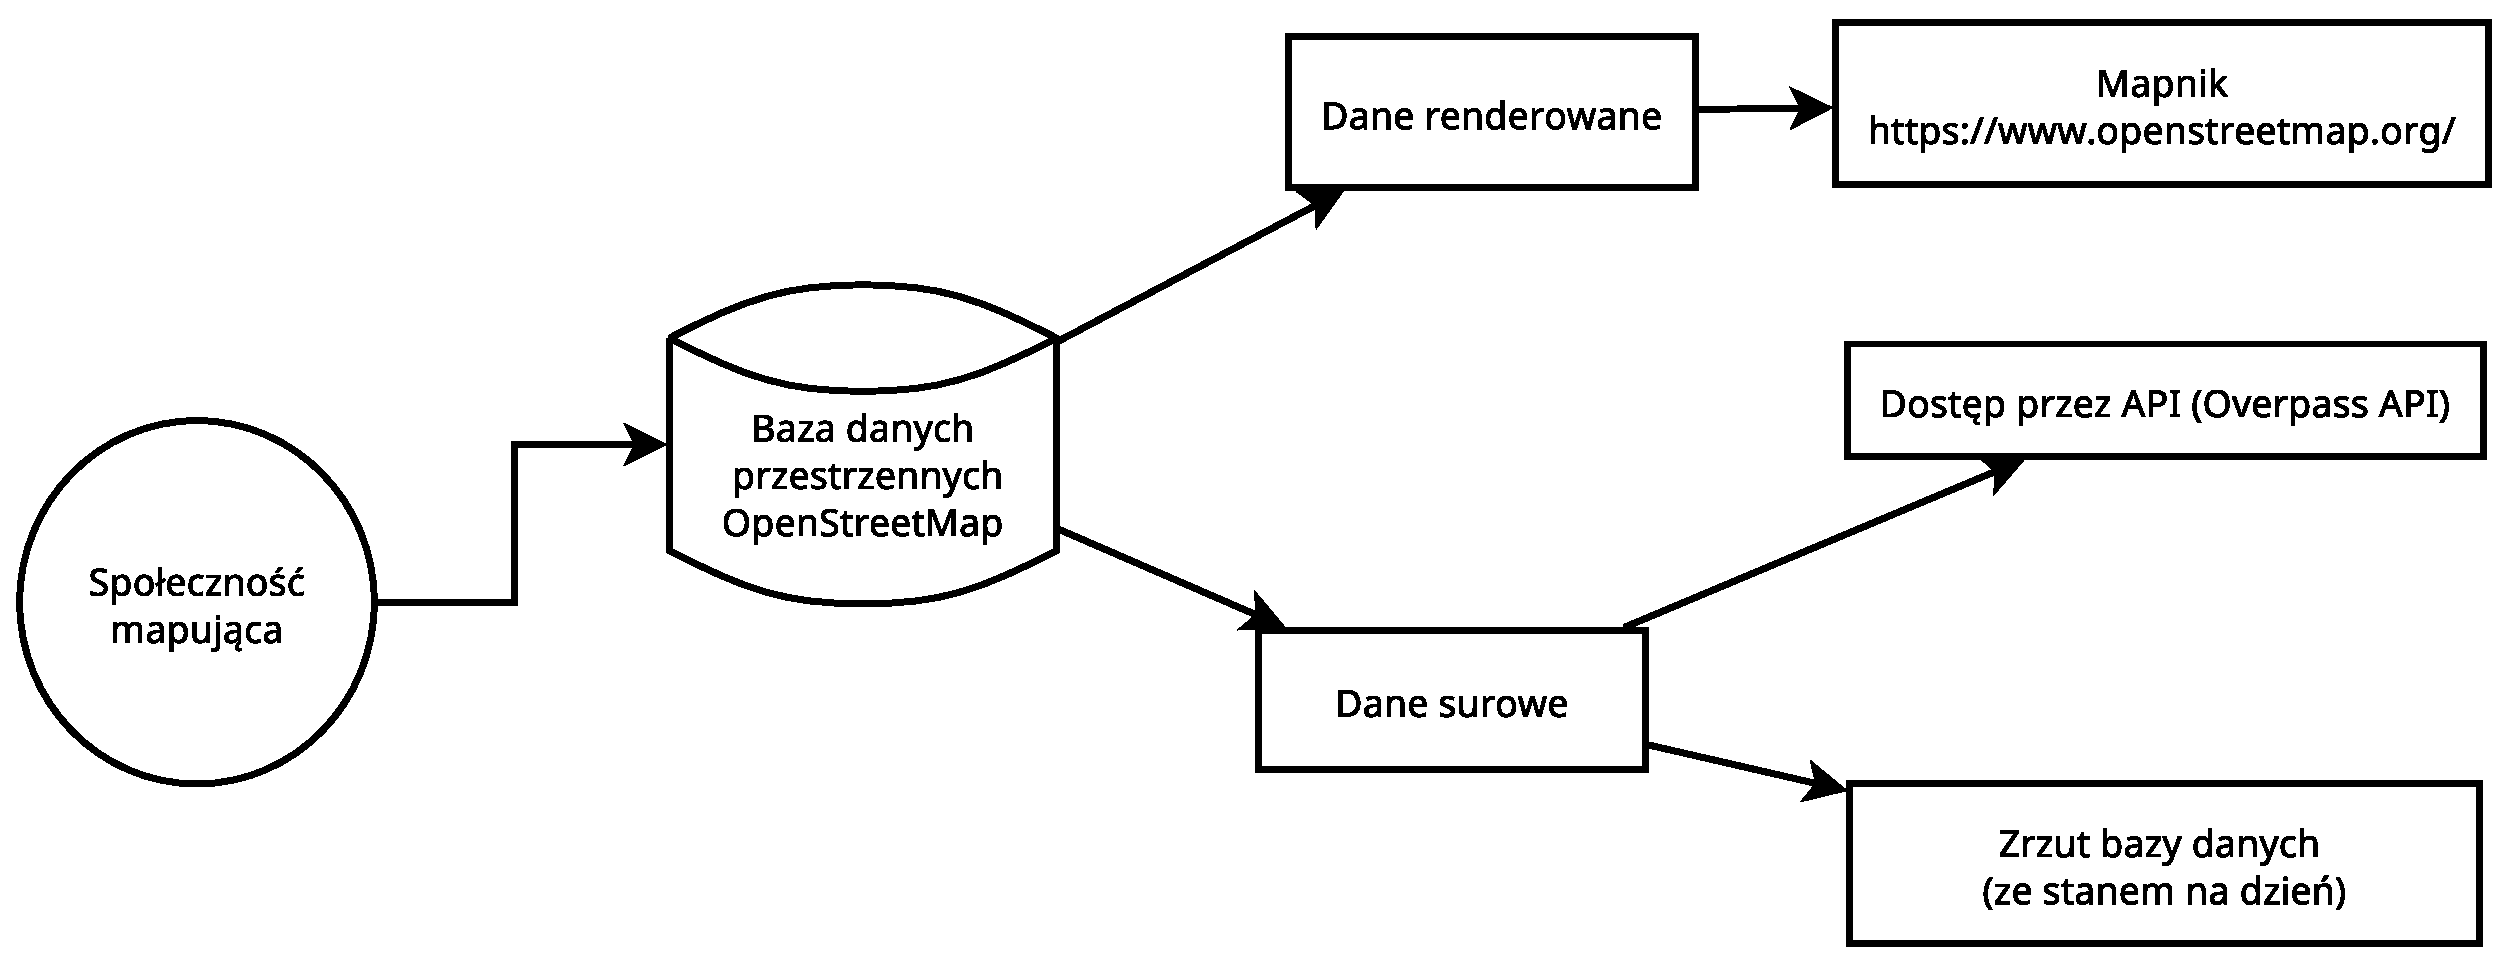
\includegraphics[width=1.3\textwidth]{/Users/mariusz/DokumentyLatex/obrazylatex/schematygislatex/obraz7.eps}
		\label{}
	\end{figure}
\end{landscape}

Dane do projektu trafiają z różnych źródeł. Projekt OSM nie jest więc wyłącznie zasilany przez dane zbierane (z rzeczywistości) przez użytkowników/osoby mapujące. Społecznościowy charakter oznacza, że dane są zarządzane przez społeczność. \par
Źródła danych w projekcie:\footnote{W przypadku OSM termin VGI \textit{(Volunteered geographic information)} nie pokazuje udziału różnorodnych danych w systemie.}
\begin{itemize}
	\item dane z ortofotomap do tworzenia obrysów,(serwis Bing ale już nie do np. określania nazw ulic)
	\item dane administracji publicznej\footnote{Aczkolwiek status danych geoportalu jest żywo dyskutowany. Analiza prawna na stronie: \url{http://ump.fuw.edu.pl/wiki/Geoportal\#Odpowied.C5.BA\_GUGiK\_08.2013\_\-\_us.C5.82ugi\_Geoportalu\_nieodp.C5.82atnie\_bez\_ogranicze.C5.84}}
	\item zbierane smartfonami (popularna aplikacja, która umożliwia szybkie edycje POI - maps.me)
	\item zbierane odbiornikami GPS
	\item rysowane \textit{ręcznie}
\end{itemize}
Nie ma więc jednolitego standardu, które określa jakiego rodzaju dane znajdują się w bazie. Sama jakość danych jest przedmiotem wielu opracowań.\footnote{Nowak Da Costa J., Bielecka E., and Całka B., Jakość danych OpenStreetMap - analiza informacji o budynkach na terenie Siedlecczyzny, „Roczniki Geomatyki [Annals of Geomatics]”, 2016, t.14, no 2 (72), ss. 193–203.}

\section{Tagi}
Każdy obiekt w OSM może być opisany jednym unikalnym kluczem i wartością. Jednak każdy obiekt może być opisany różnym zestawem kluczy i wartości. System pozwala na precyzyjne opisanie obiektów, ale nie zawsze jest to praktykowane. Typowy błąd można przedstawić na przykładzie klucza \textit{building}.\par
Dla klucza \textbf{building} istnieje 10799 różnorodnych wartości\footnote{\url{https://taginfo.openstreetmap.org/keys/building\#values}}
jednak najczęściej używana (81 \%) to wartość - \textit{yes}. Pojawiają się też takie wartości jak - \textit{?} (321 razy), - \textit{fixme}, - \textit{unknown} itd. \par
W celu wyodrębnienia tych wszystkich danych została użyta metoda precyzyjna - wyodrębnienia najpopularniejszych tagów building (w nomenklaturze building_(\textit{nazwa wartości})) i tag ogólny, który zbiera elementy nie sprecyzowane wcześniej (building).
\chapter{Pobieranie danych}



\section{Dane Polska}

Pobieranie danych Openstreemap ze strony \url{http://download.geofabrik.de/europe/poland.html}. \par
W środowisku Linux
\noindent Pobierz najnowsze dane:
\begin{lstlisting} [language=bash, caption={Komenda bash}]
$ wget http://download.geofabrik.de/europe/poland-latest.osm.pbf
\end{lstlisting}

\section{Dane gminy}

Podstawą do stworzenia bazy danych zmian administracyjnych gmin, oraz danych o metropoliach była strona Tomasza Żółtaka  \url{https://tomek.zozlak.org/inne/podz_teryt/podz_teryt.php}

\chapter{Przygotowanie bazy danych.}

\section{Konfiguracja Postgresql}

Stworzenie bazy danych postgres z zarejestrowanymi dodatkami: \begin{itemize}
	\item postgis (rozszerzenie przestrzenne)
	\item hstore (przechowywanie rzadko używanych tagów)
	\item pgrouting (wyznaczanie tras)
\end{itemize}
Baza danych "gis-osm". W schematach graficznych może funkcjonować jako gis-access.

W środowisku Linux
\noindent Po zainstalowaniu i konfiguracji Postgresql (użytkownik Postgres - przełączenie się na użytkownika ). Kolejność komend - przełączenie się na użytkownika postgres, zalogowanie się do środowiska postgresql, usunięcie istniejącej bazy danych gis-osm, wyjście ze środowiska, utworzenie nowej bazy danych gis-osm, utworzenie nowych dodatków w bazie.

\begin{lstlisting}[language=bash]
sudo -u postgres -i
psql
DROP DATABASE gis-osm
\q
createdb gis-osm
psql -d gis-osm -c 'CREATE EXTENSION postgis; CREATE EXTENSION hstore; 	CREATE EXTENSION pgrouting;'
\end{lstlisting}

\section{Upgrade bazy postgresql lub postgis/pgrouting}

Najprostszą metodą upgradu do pełnej wersji postgresql jest backup bazy, zatrzymanie serwera (w Linuksie np. sudo systemctl stop postgresql.service) usunięcie katalogu /var/lib/postgres/data/ . Następnie inicjalizacja nowej bazy postgres i uruchomienie serwera postresql. \par
\subsection{Aktualizacja pakietów w Arch Linux}
Nowe wersje oprogramowania mogą wymagać przebudowania pakietów. Najnowsze wersje postgisa i pgroutingu znajdują się w serwisie github. Można spróbować ręcznej aktualizacji pakietów wykorzystując system budowy pakietów Arch Linux - aur. Przy użyciu komendy  yaourt --m-arg "--skippgpcheck" -S . Pominięte zostanie sprawdzenie sumy kontrolnej, dzięki temu można podmienić np. wersję pakietu do zbudowania.  (to do: yaourt nie jest już wspierany, używana powinna być metoda dla menadżera - trizen)

\section{Narzędzia do konwersji danych Openstreetmap}

\subsection{Pełne dane}

Do stworzenia bazy danych postgres z danymi osm użyto \url{https://github.com/openstreetmap/osm2pgsql}.\par
W efekcie uzyskujemy 4 tabele:
\begin{itemize}
	\item planet_osm_point, 
	\item planet_osm_line, 
	\item planet_osm_roads,
	\item planet_osm_polygon
\end{itemize}

Przygotowany i zmodyfikowany plik default.style znajduje się w
Dodatku A.

\noindent Po stworzeniu lub modyfikacji pliku default.style można przystąpić do wypełniania danymi osm:
\begin{lstlisting}[language=bash,caption={Komenda bash}]]
osm2pgsql -s -U postgres --hstore -d gis-osm 
 --style /home/mariusz/default.style 
 --multi-geometry --extra-attributes poland-latest.osm.pbf
\end{lstlisting}
Proces może trwać ponad 2 godziny i potrzebnej jest co najmniej 8GB pamięci. Program w październiku 2017 roku był w wersji 0.95-dev.

Potencjalny skrypt do aktualizacji danych z osm
\begin{lstlisting}[ language=bash, caption={Skrypt bash}]
#!/bin/sh
DATA=`date +%j`
DATA1=`expr $DATA + 20`
# bashu sprawdza dzień i dodaje przesunięcie
wget http://download.geofabrik.de/europe/poland-updates/000/001/$DATA1.osc.gz
osm2pgsql --append -s --hstore -d gis-access-ok --style /home/mariusz/default.style --multi-geometry $DATA1.osc.gz
\end{lstlisting}


\begin{landscape}
\begin{figure}[htp]
\caption{Pełne dane OSM.}
\centering
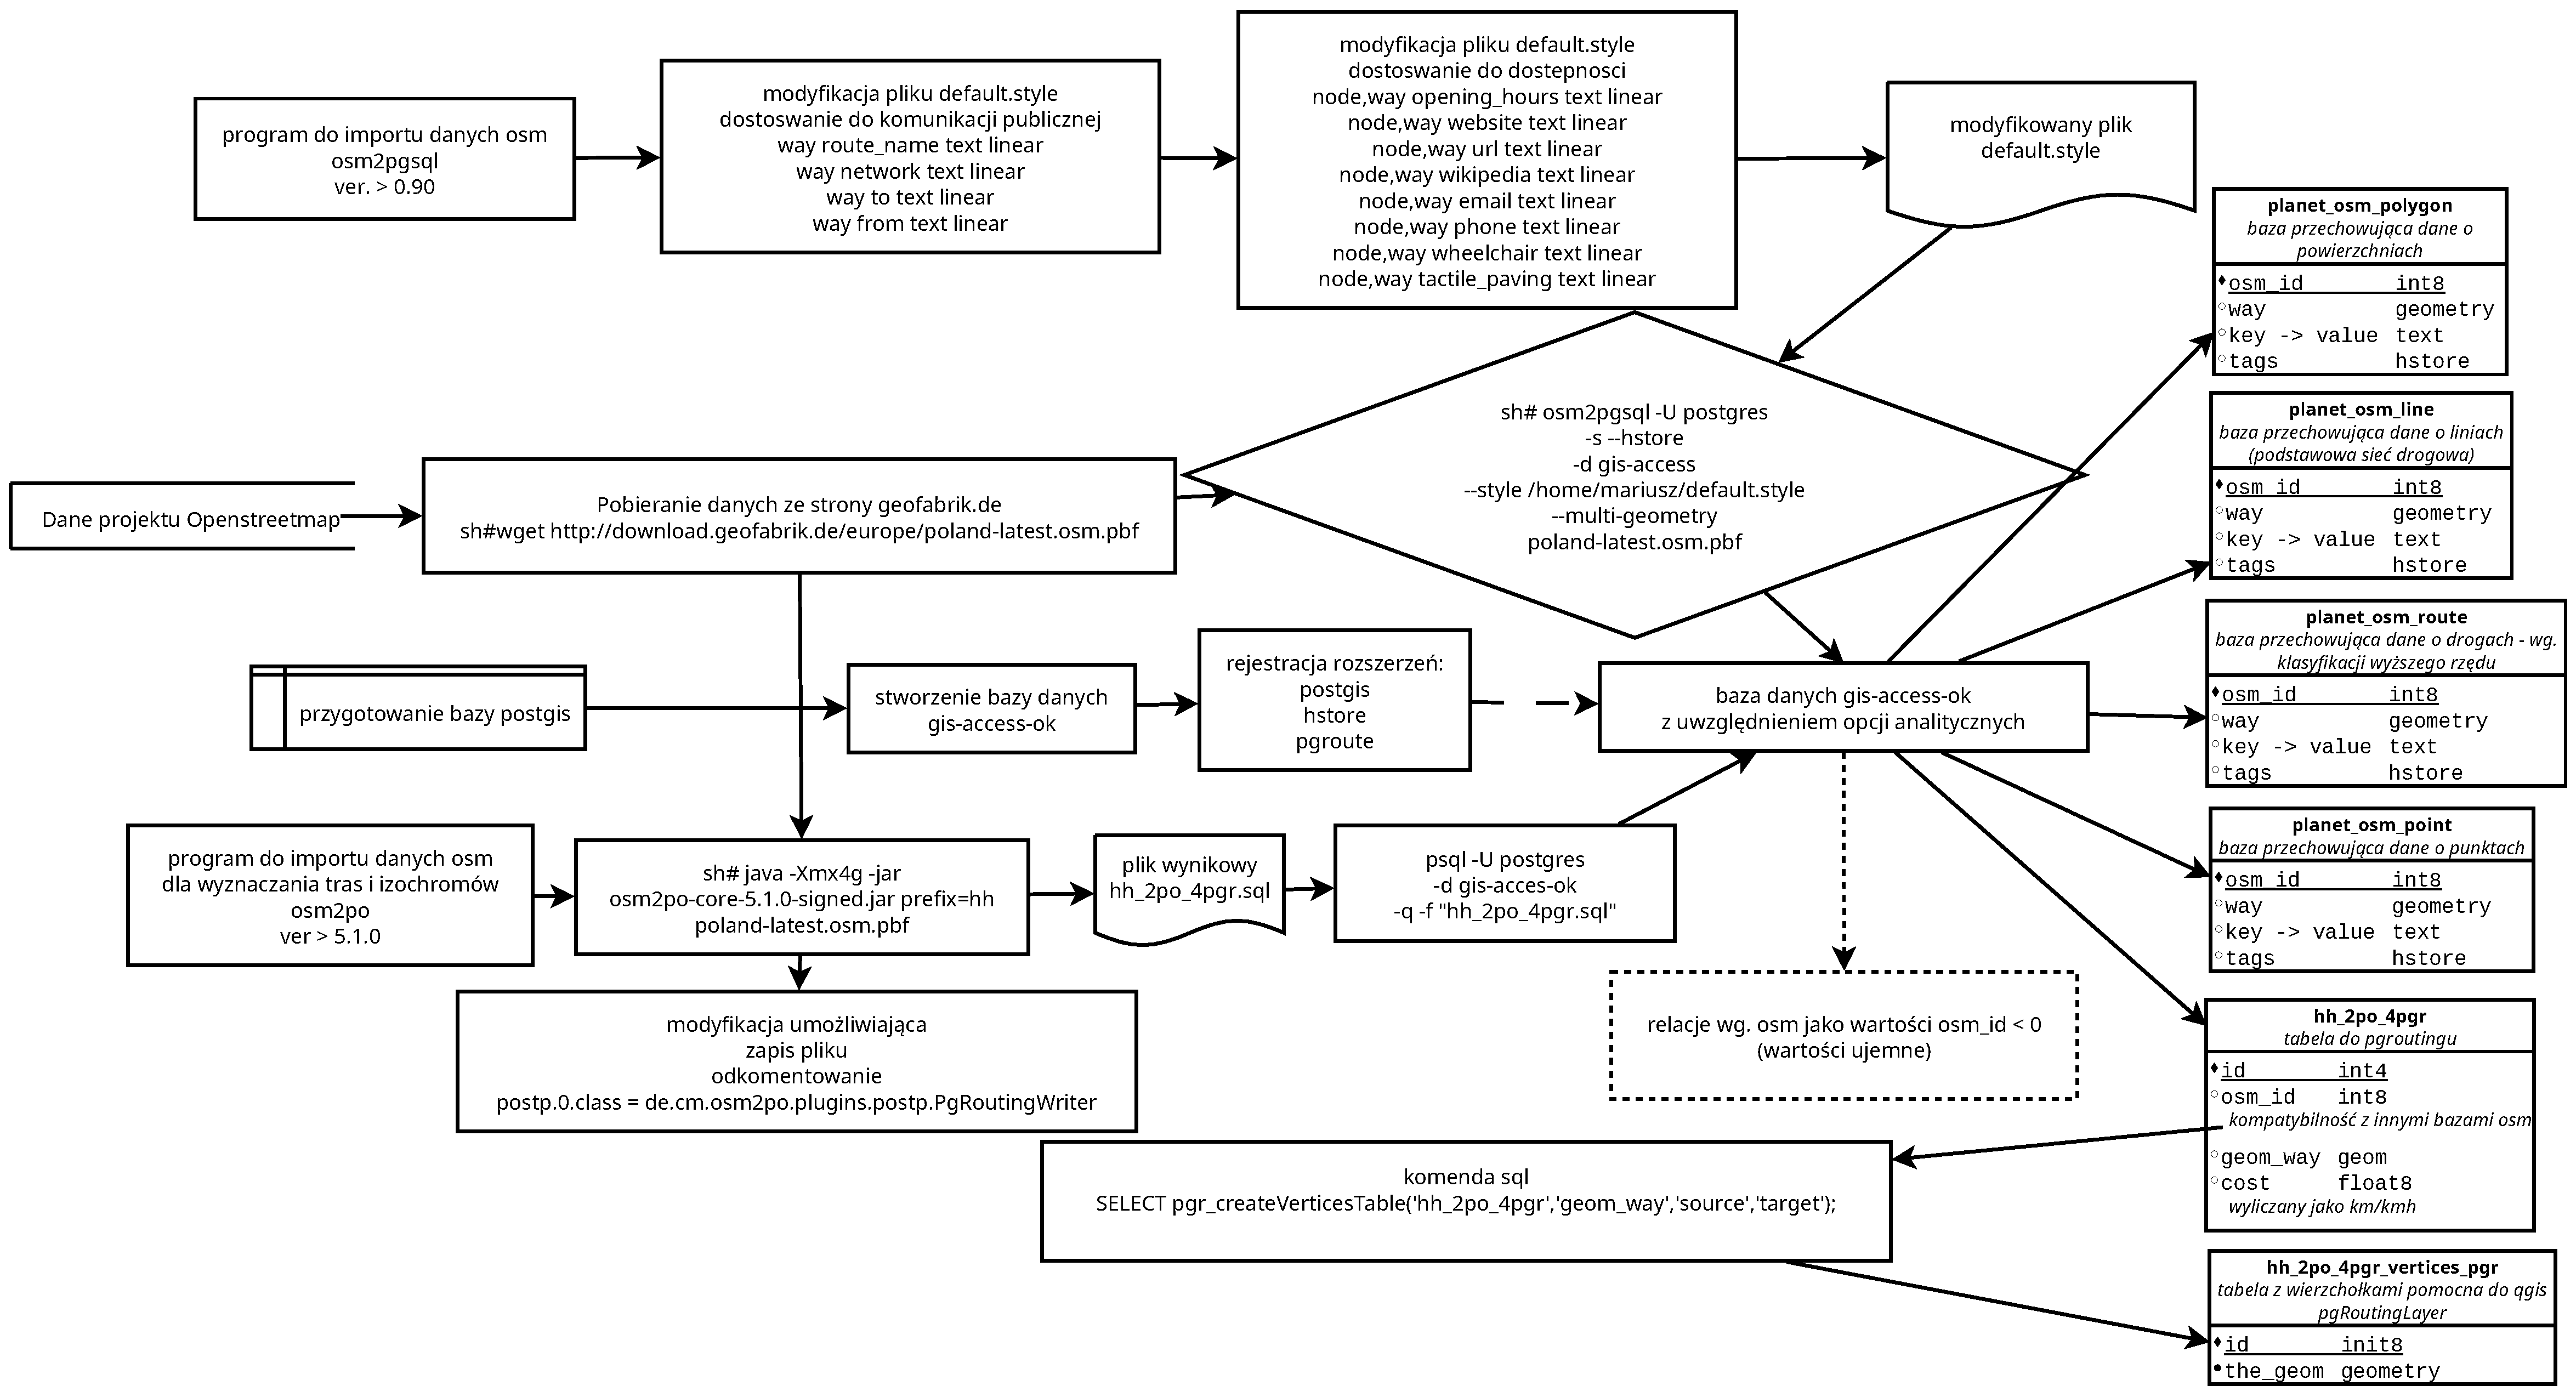
\includegraphics[width=1.6\textwidth]{/Users/mariusz/DokumentyLatex/obrazylatex/schematygislatex/obraz1a.eps}
\label{}
\end{figure}
\end{landscape}

Pełen schemat danych prezentuje Tabela \ref{table:1}





	\begin{longtable}{l|p{4.2cm}|l}

	\caption{Struktura tabeli w bazie postgresql}
	\label{table:1}
\endfirsthead	
		Nazwa klucza (key) & typ zmiennej & charakterystyka   \\\hline
	 osm_id & bigint & unikalne id \\
	access & text & \\
		addr:housename    & text     &      \\
		addr:housenumber   & text           \\
		addr:interpolation & text           \\\hline
		admin\_level       & text     & dane granic administracyjnych itp.      \\\hline
		aerialway          & text           \\
		aeroway            & text           \\
		amenity            & text     & Typy wartości (\textit{value}) w załączniku C      \\\hline
		area               & text           \\
		barrier            & text           \\
		bicycle            & text           \\
		brand              & text           \\
		bridge             & text           \\
		boundary           & text           \\
		building           & text  & Typy wartości (\textit{value}) w załączniku C          \\\hline
		capital            & text           \\
		construction       & text           \\
		covered            & text           \\
		culvert            & text           \\
		cutting            & text           \\
		denomination       & text           \\
		disused            & text           \\
		ele                & text           \\
		embankment         & text           \\
		foot               & text           \\
		generator:source   & text           \\
		harbour            & text           \\
		highway            & text           \\
		historic           & text    & Typy wartości (\textit{value}) w załączniku C        \\\hline
		horse              & text           \\
		intermittent       & text           \\
		junction           & text           \\\hline
		landuse            & text    & Typy wartości (\textit{value}) w załączniku C        \\
		layer              & text           \\
		leisure            & text    & Typy wartości (\textit{value}) w załączniku C        \\\hline
		lock               & text           \\
		man\_made          & text    & Typy wartości (\textit{value}) w załączniku C        \\
		military           & text    & Typy wartości (\textit{value}) w załączniku C        \\
		motorcar           & text           \\
		name               & text           \\
		natural            & text  & Typy wartości (\textit{value}) w załączniku C          \\
		office             & text    & Typy wartości (\textit{value}) w załączniku C        \\
		oneway             & text           \\
		operator           & text           \\
		place              & text           \\
		population         & text           \\
		power              & text           \\
		power\_source      & text           \\
		public\_transport  & text           \\
		railway            & text           \\
		ref                & text           \\
		religion           & text           \\
		route              & text           \\
		service            & text           \\
		shop               & text    & Typy wartości (\textit{value}) w załączniku C        \\
		sport              & text           \\
		surface            & text           \\
		toll               & text           \\
		tourism            & text  & Typy wartości (\textit{value}) w załączniku C          \\
		tower:type         & text           \\
		tunnel             & text           \\
		water              & text           \\
		waterway           & text           \\
		wetland            & text           \\
		width              & text           \\
		wood               & text           \\\hline
		opening\_hours     & text  & wyodrębnione        \\
		website            & text           \\
		url                & text           \\
		wikipedia          & text           \\
		email              & text           \\
		phone              & text           \\\hline
		wheelchair         & text     & niepełnosprawni ruchowo      \\
		tactile\_paving    & text           \\\hline
		z\_order           & integer        \\
	\textbf{	tags}               &\textbf{ hstore}  & tagi sporadyczne       \\\hline
	\textbf{	way            }    & \textbf{geometry(Point 3857)}
	\end{longtable}


\subsection{Dane punktowe - POI}

Do konwersji użyto programu \url{https://github.com/MorbZ/OsmPoisPbf}. wymaga on zainstalowanego środowiska Java.
\begin{lstlisting}[ language=bash]
$ java -Xmx4g -jar osmpois.jar -p 4 --filterFile filter.txt 
	--outputTag name,wheelchair,url,website,opening_hours
	 -r -u poland-latest.osm.pbf
\end{lstlisting}
atrybuty -r i -u poszerzają wyszukiwanie o dane o relacjach.\par
Zmodyfikowany plik filter.txt znajduje się w Dodatku B.\par
Efektem działania programu jest plik poland-latest.csv. Separatorem pola jest znak |. W trakcie importu do programu QGIS należy zamienić miejscami X i Y, oraz ustawić projekcję - 4326.
Plik posiada następującą strukturę: \par


\begin{tabular}{|l|l|}

	\hline 
Nazwa kolumny	& Typ informacji \\ 
	\hline\hline
id	&  unikalny identyfikator\\ 
	\hline 
osm_id	&  kod zgodny z bazą OSM\\ 
	\hline 
kod_osm	& numer tagu wg pliku filter.txt \\ 
	\hline 

\end{tabular} \\



\begin{figure}[h]
\caption{Schemat przetwarzania informacji słownikowej OSM - OZK.}
\centering
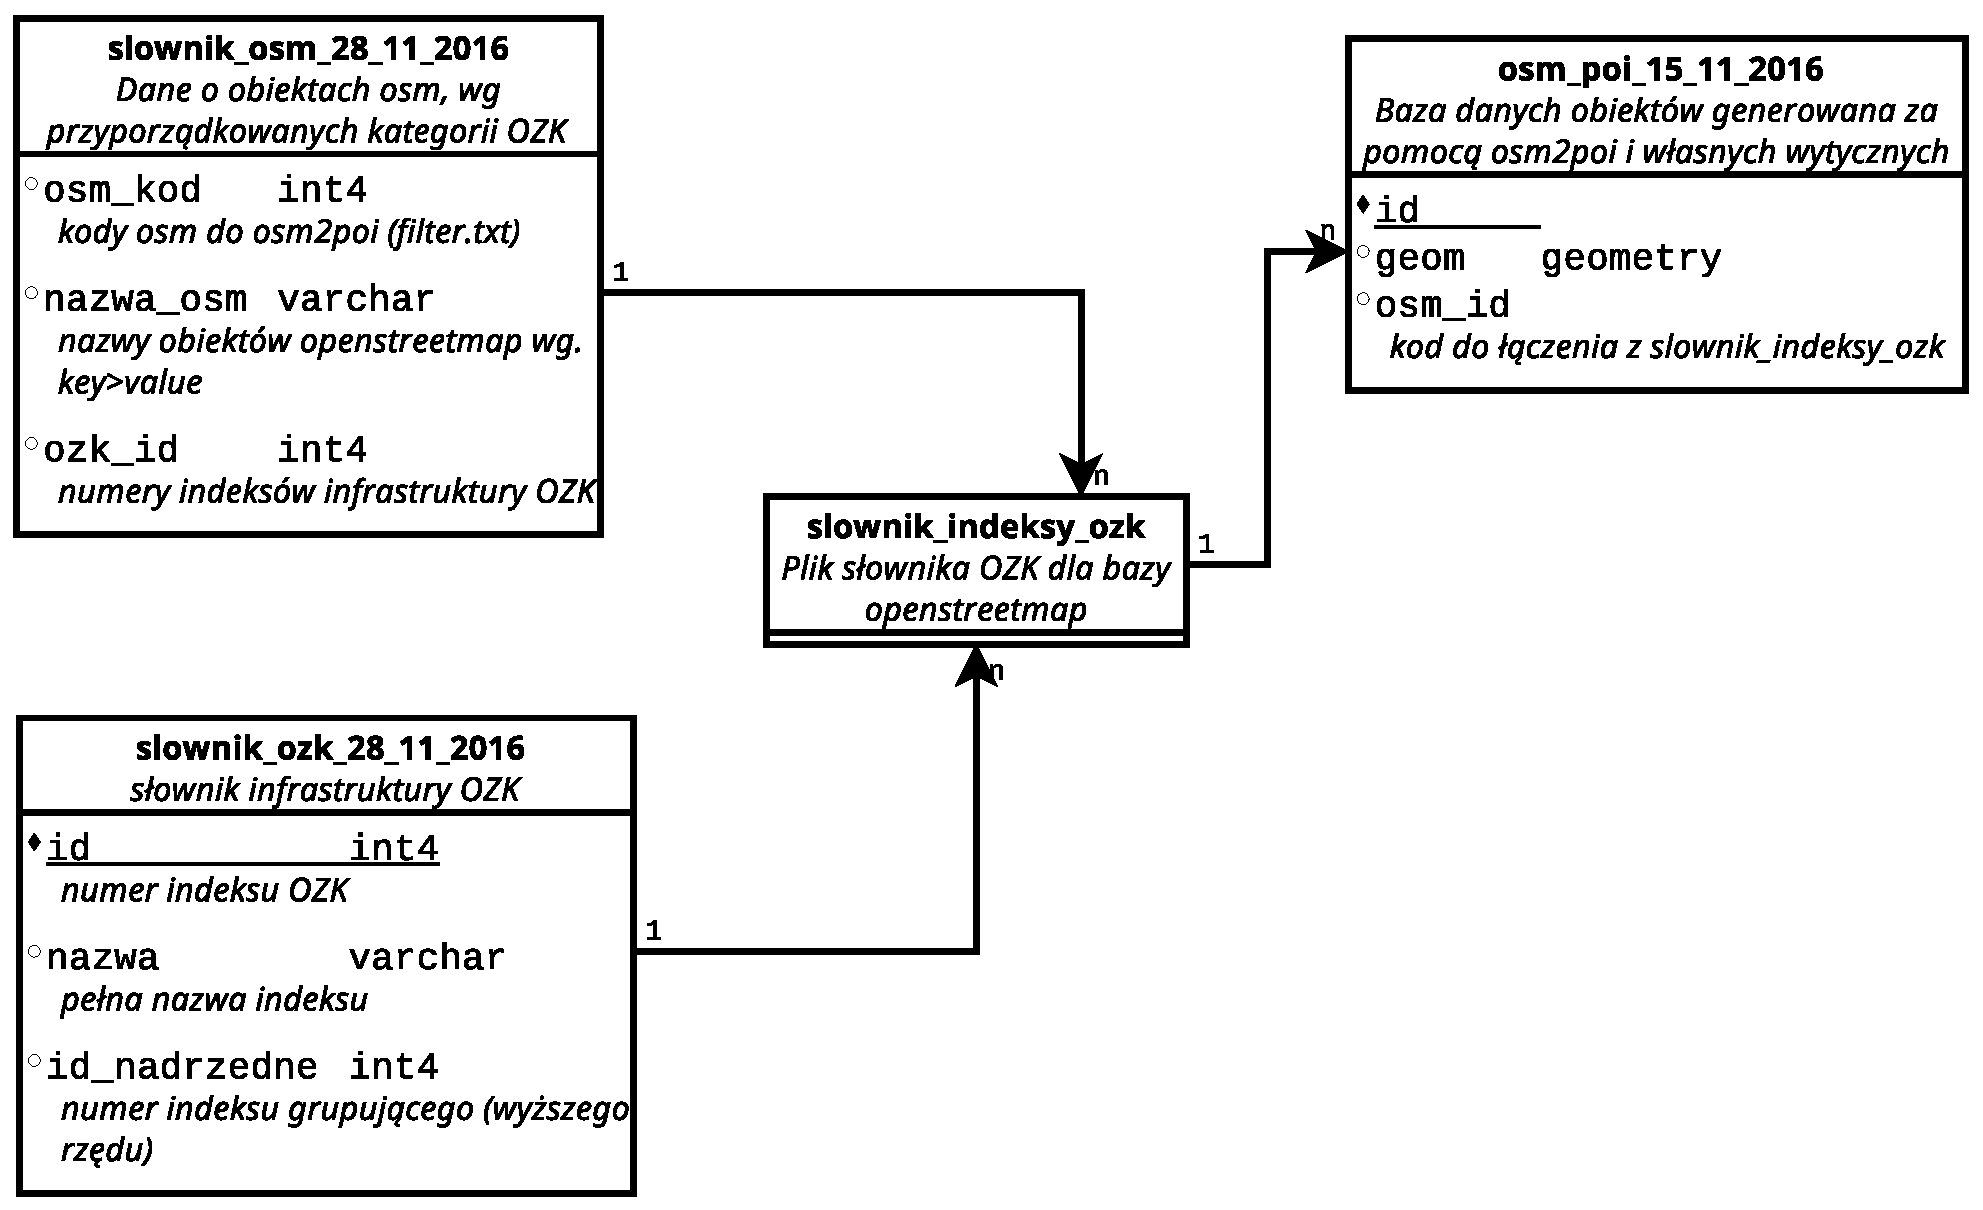
\includegraphics[width=1\textwidth]{/Users/mariusz/DokumentyLatex/obrazylatex/schematygislatex/obraz3a.eps}
	
\label{}
	
\end{figure}



W celu przypisania kodów_osm do indeksów infrastruktury można użyć pliku pliku sl_ozk_osm_indeksy_srednik_pelne_3_poziomy.csv
Lub też użyć komendy
\begin{lstlisting}[ language=SQL]
select *
from osm_poi_7_8_2017
left join slownik_indeksy_ozk
on osm_poi_7_8_2017.field_1::text = slownik_indeksy_ozk.osm_kod::text
\end{lstlisting}
lub też od razu stworzyć nową bazę powiększoną o pola słownika i poprawionymi nazwami pól
\begin{lstlisting}[ language=SQL]
select 
field_2 as osm_id, 
field_3 as lang, 
field_4 as lat, 
field_5 as nazwa, 
field_6 as wheelchair, 
field_7 as url, 
field_8 as website, 
field_9 as opening_hours,
osm_poi_7_8_2017.geom,
osm_poi_7_8_2017.id,
osm_kod, 
nazwa_osm,
indeksy_ozk_aktualne_nazwa, 
indeksy_ozk_aktualne_id_nadrzedne
into public.osm_poi_7_8_2017_ozk
from osm_poi_7_8_2017
left join slownik_indeksy_ozk
on osm_poi_7_8_2017.field_1::text = slownik_indeksy_ozk.osm_kod::text


\end{lstlisting}

W przypadku problemów z primary key w nowej bazie można usunąć kolumnę z id i na nową wygenerować primary key

\begin{lstlisting}[language=SQL]
	alter table osm_poi_7_8_2017_ozk Drop column id;
	alter table osm_poi_7_8_2017_ozk add column id serial primary key;
\end{lstlisting}

\begin{landscape}
	\begin{figure}[htp]
		\caption{Schemat przetwarzania informacji o punktach.}
		\centering
		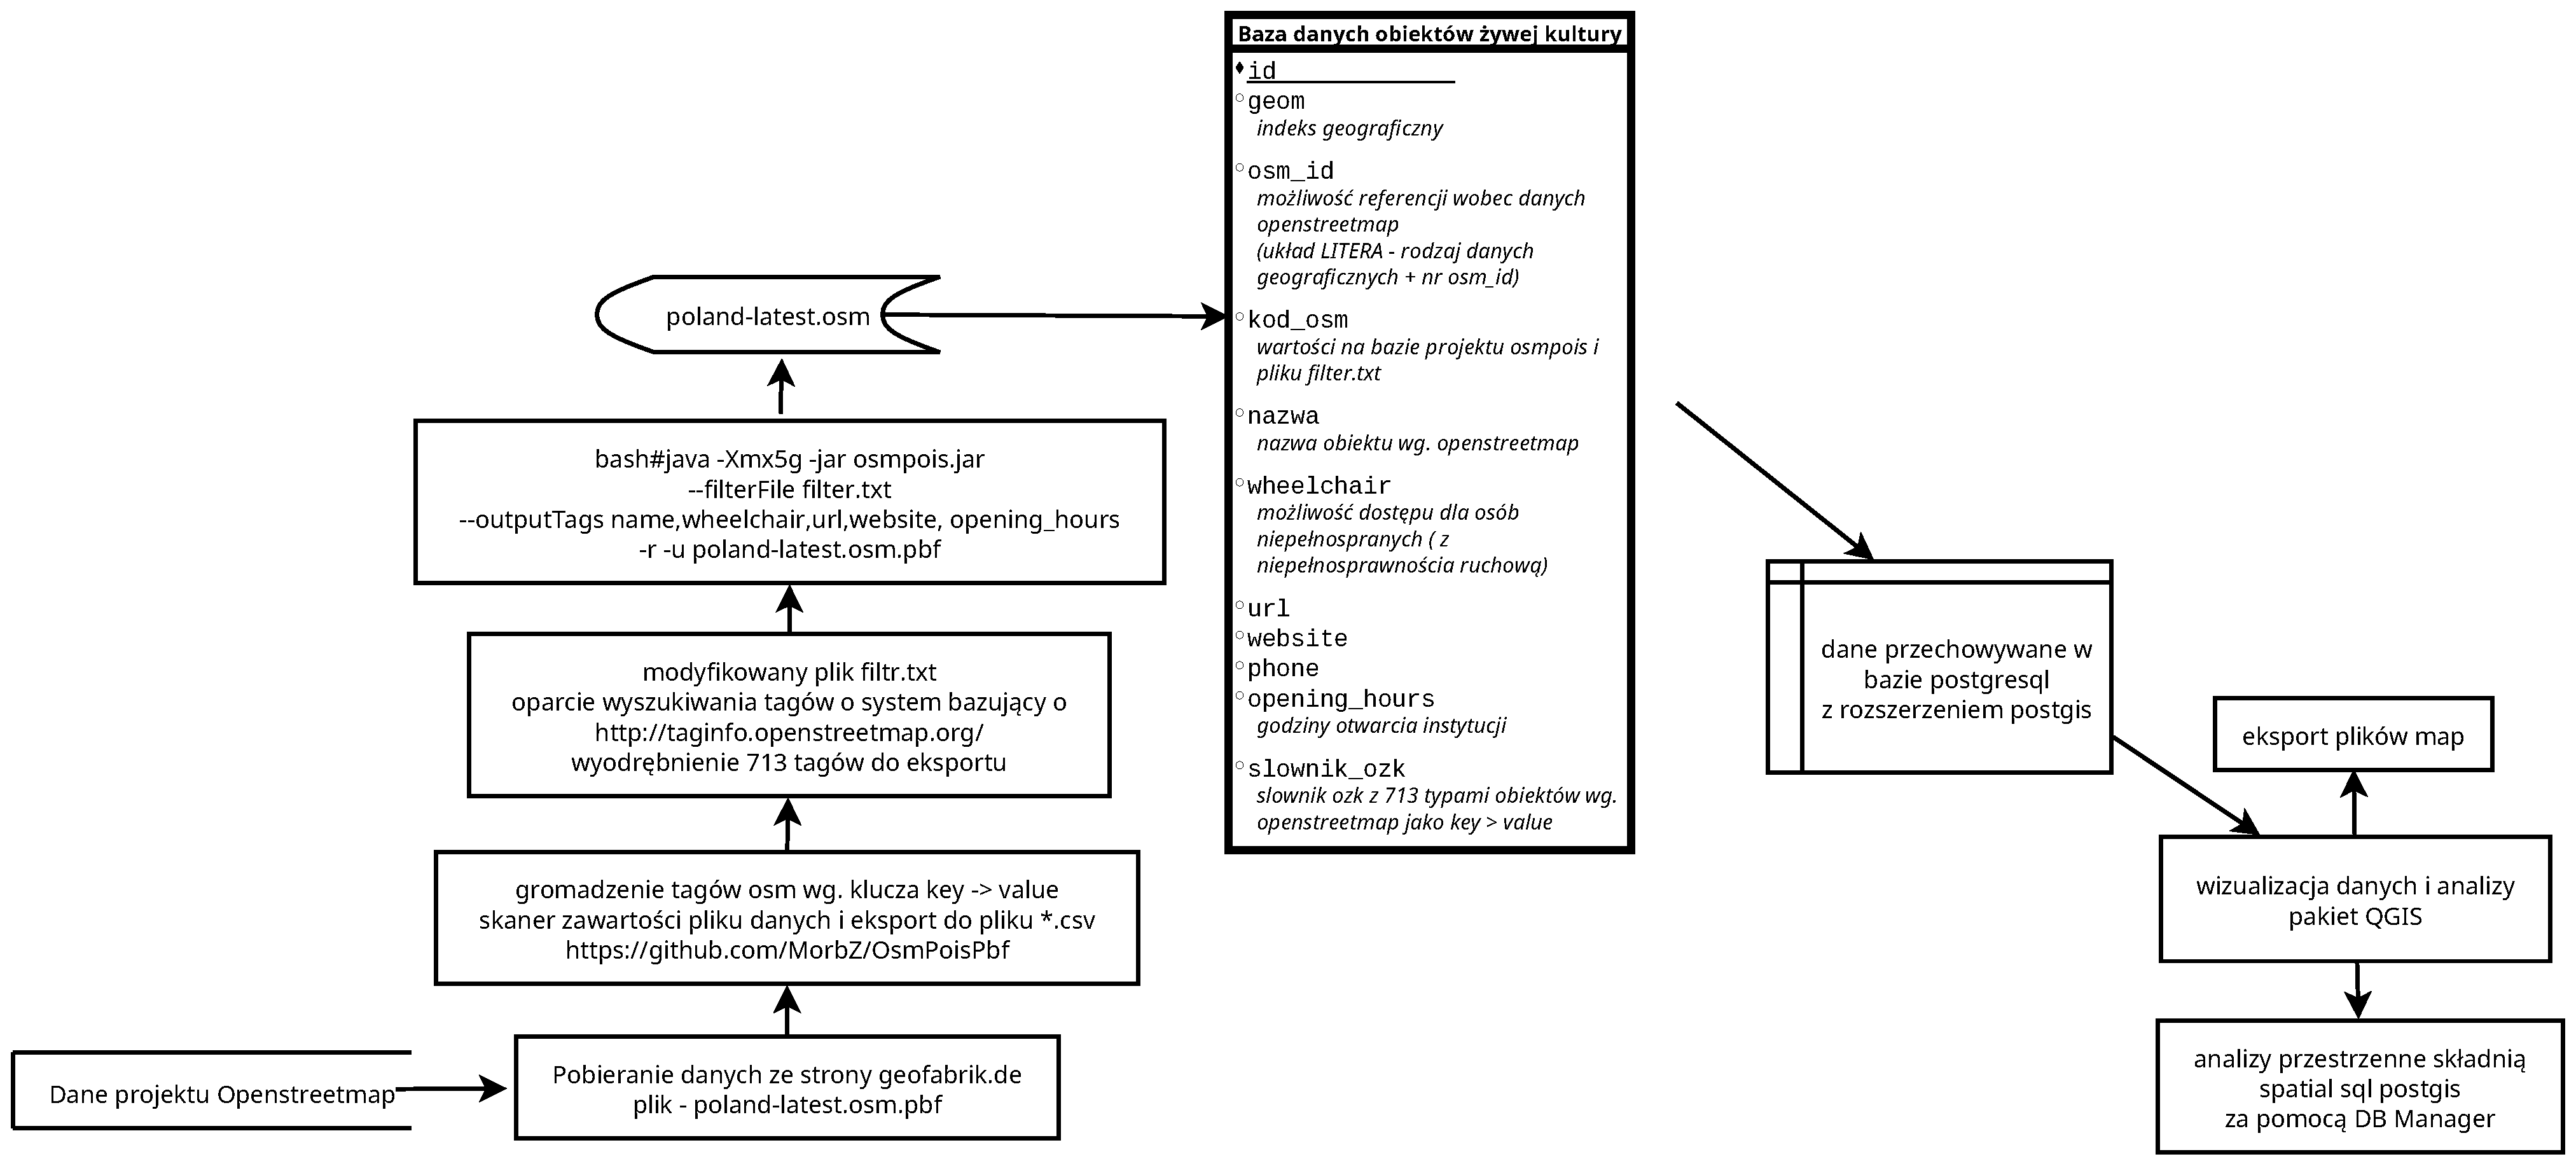
\includegraphics[width=1.6\textwidth]{/Users/mariusz/DokumentyLatex/obrazylatex/schematygislatex/obraz2a.eps}
		
		\label{}
		
	\end{figure}
\end{landscape}
\subsection{Wyznaczanie tras - pgrouting.}

NOTATKA! Twórcy pgrouging używają do konwersji danych z osm osm2pgrouting - brakuje niestety tego programu w Arch. \par

Sieć drogowa wygenerowana za pomocą osm2pgsql nie pozwala na używanie rozszerzenia pgrouting. Konwersję dróg do formatu wektorowego wykonać można w programie osm2po \url{http://osm2po.de/}.\par
Efektem działania programu jest wygenerowanie pliku z bazą danych (rozszerzenie sql- hh2po4pgr.sql):

\begin{lstlisting}[ language=bash]
$ java -Xmx4g -jar osm2po-core-5.1.0-signed.jar 
	 prefix=hh poland-latest-osm.pbf
\end{lstlisting}
Aby móc zapisać plik sql należy odkomentować następujący wiersz w pliku  osm2po.config
\begin{lstlisting}[ language=bash]
postp.0.class = de.cm.osm2po.plugins.postp.PgRoutingWriter
\end{lstlisting}

Powstały plik można załączyć do bazy postgresql. Czynność wykonujemy komendą:
\begin{lstlisting}[ language=bash]
psql -U postgres -d gis-osm -q -f hh2po4pgr.sql
\end{lstlisting}
Po załadowaniu pliku należy jeszcze stworzyć tablicę wektorów, aby móc używać danych w programie QGIS. Czynność wykonujemy w bazie postgresql.
\begin{lstlisting}[ language=SQL, caption={Tworzenie tabeli wektorów}]
SELECT pgr_createVerticesTable('hh2po4pgr','geom_way','source','target');
\end{lstlisting}
W powstałej tabeli z danymi hh2po4pgr - kolumna cost - jest wyliczana jako 
\( \displaystyle \frac{km}{\frac{km}{h}} \)
Ostatnią czynnością porządkową jest przekształcenie układu współrzędnych z 4326 na 2180, który pozwoli na analizy odległości w metrach.

\section{Projekcja w locie}


Problem z projekcją układów współrzędnych, który pojawia się w analizach pokazuje film \url{https://www.youtube.com/watch?feature=youtu.be&v=kIID5FDi2JQ&app=desktop} \par
Dodatkowe źródła informacji o postgis:
\begin{itemize}
	\item \url{http://workshops.boundlessgeo.com/postgis-intro/index.html}
\end{itemize} \par
Dane, w celu wykonywania obliczeń należy przekształcić do układu współrzędnych EPSG 2180. W programie QGIS można skorzystać z projekcji w locie. Dane można przekształcić w bazie Postgresql. \\

\begin{table}[h]
	\centering
\begin{tabular}{|p{3cm}|p{3.2cm}|l|}

	\hline 
\textbf{Typ projekcji}	& \textbf{jednostka miary} & \textbf{gdzie używany}\\ 
	\hline 
\textbf{EPSG 3857} (WGS84)	&  metry & osm2pqsl\\ 
	\hline 
\textbf{EPSG 4326} (WGS84)	&  w stopniach &  osm2po (do wyznaczania tras)\\ 
	\hline 
\textbf{EPSG 2180 }	(ETRS89/CS92	) & metry & docelowy \\ 
	\hline 
\end{tabular} 
\end{table}
\chapter{Praca na danych Openstreetmap.}
\section{Przetwarzanie danych powierzchniowych.}

W celu wyodrębnienia pliku z informacjami o powierzchniach terenów zielonych zostało użyte następujące polecenie:
\begin{lstlisting}[ language=SQL, caption={Obrysy terenów zielonych}]
select * 
from planet_osm_polygon
where (landuse IN ('park' , 'garden' ,'forest' , 'village_garden' , 'village_green') OR 
leisure IN ( 'park' , 'nature_reserve', 'garden' ) OR 
planet_osm_polygon.natural IN ( 'forest' , 'scrub', 'grassland', 'wood' ) OR boundary = 'national_park')
\end{lstlisting}


Obszary wodne posiadają następujące parametry:
\begin{lstlisting}[ language=SQL, caption={Obrysy akwenów wodnych}]
select * 
from planet_osm_polygon
where (landuse IN ( 'stream', 'water', 'pond', 'reservoir') OR 
water IN ('river', 'lake', 'canal', 'stream', 'reservoir') OR 
waterway IN ('river', 'riverbank', 'stream', 'stream;river', 'water' ) OR 
planet_osm_polygon.natural IN ('water'))
\end{lstlisting}

\begin{landscape}
\begin{figure}[htp]
	\caption{Schemat przetwarzania informacji o powierzchniach.}
\centering
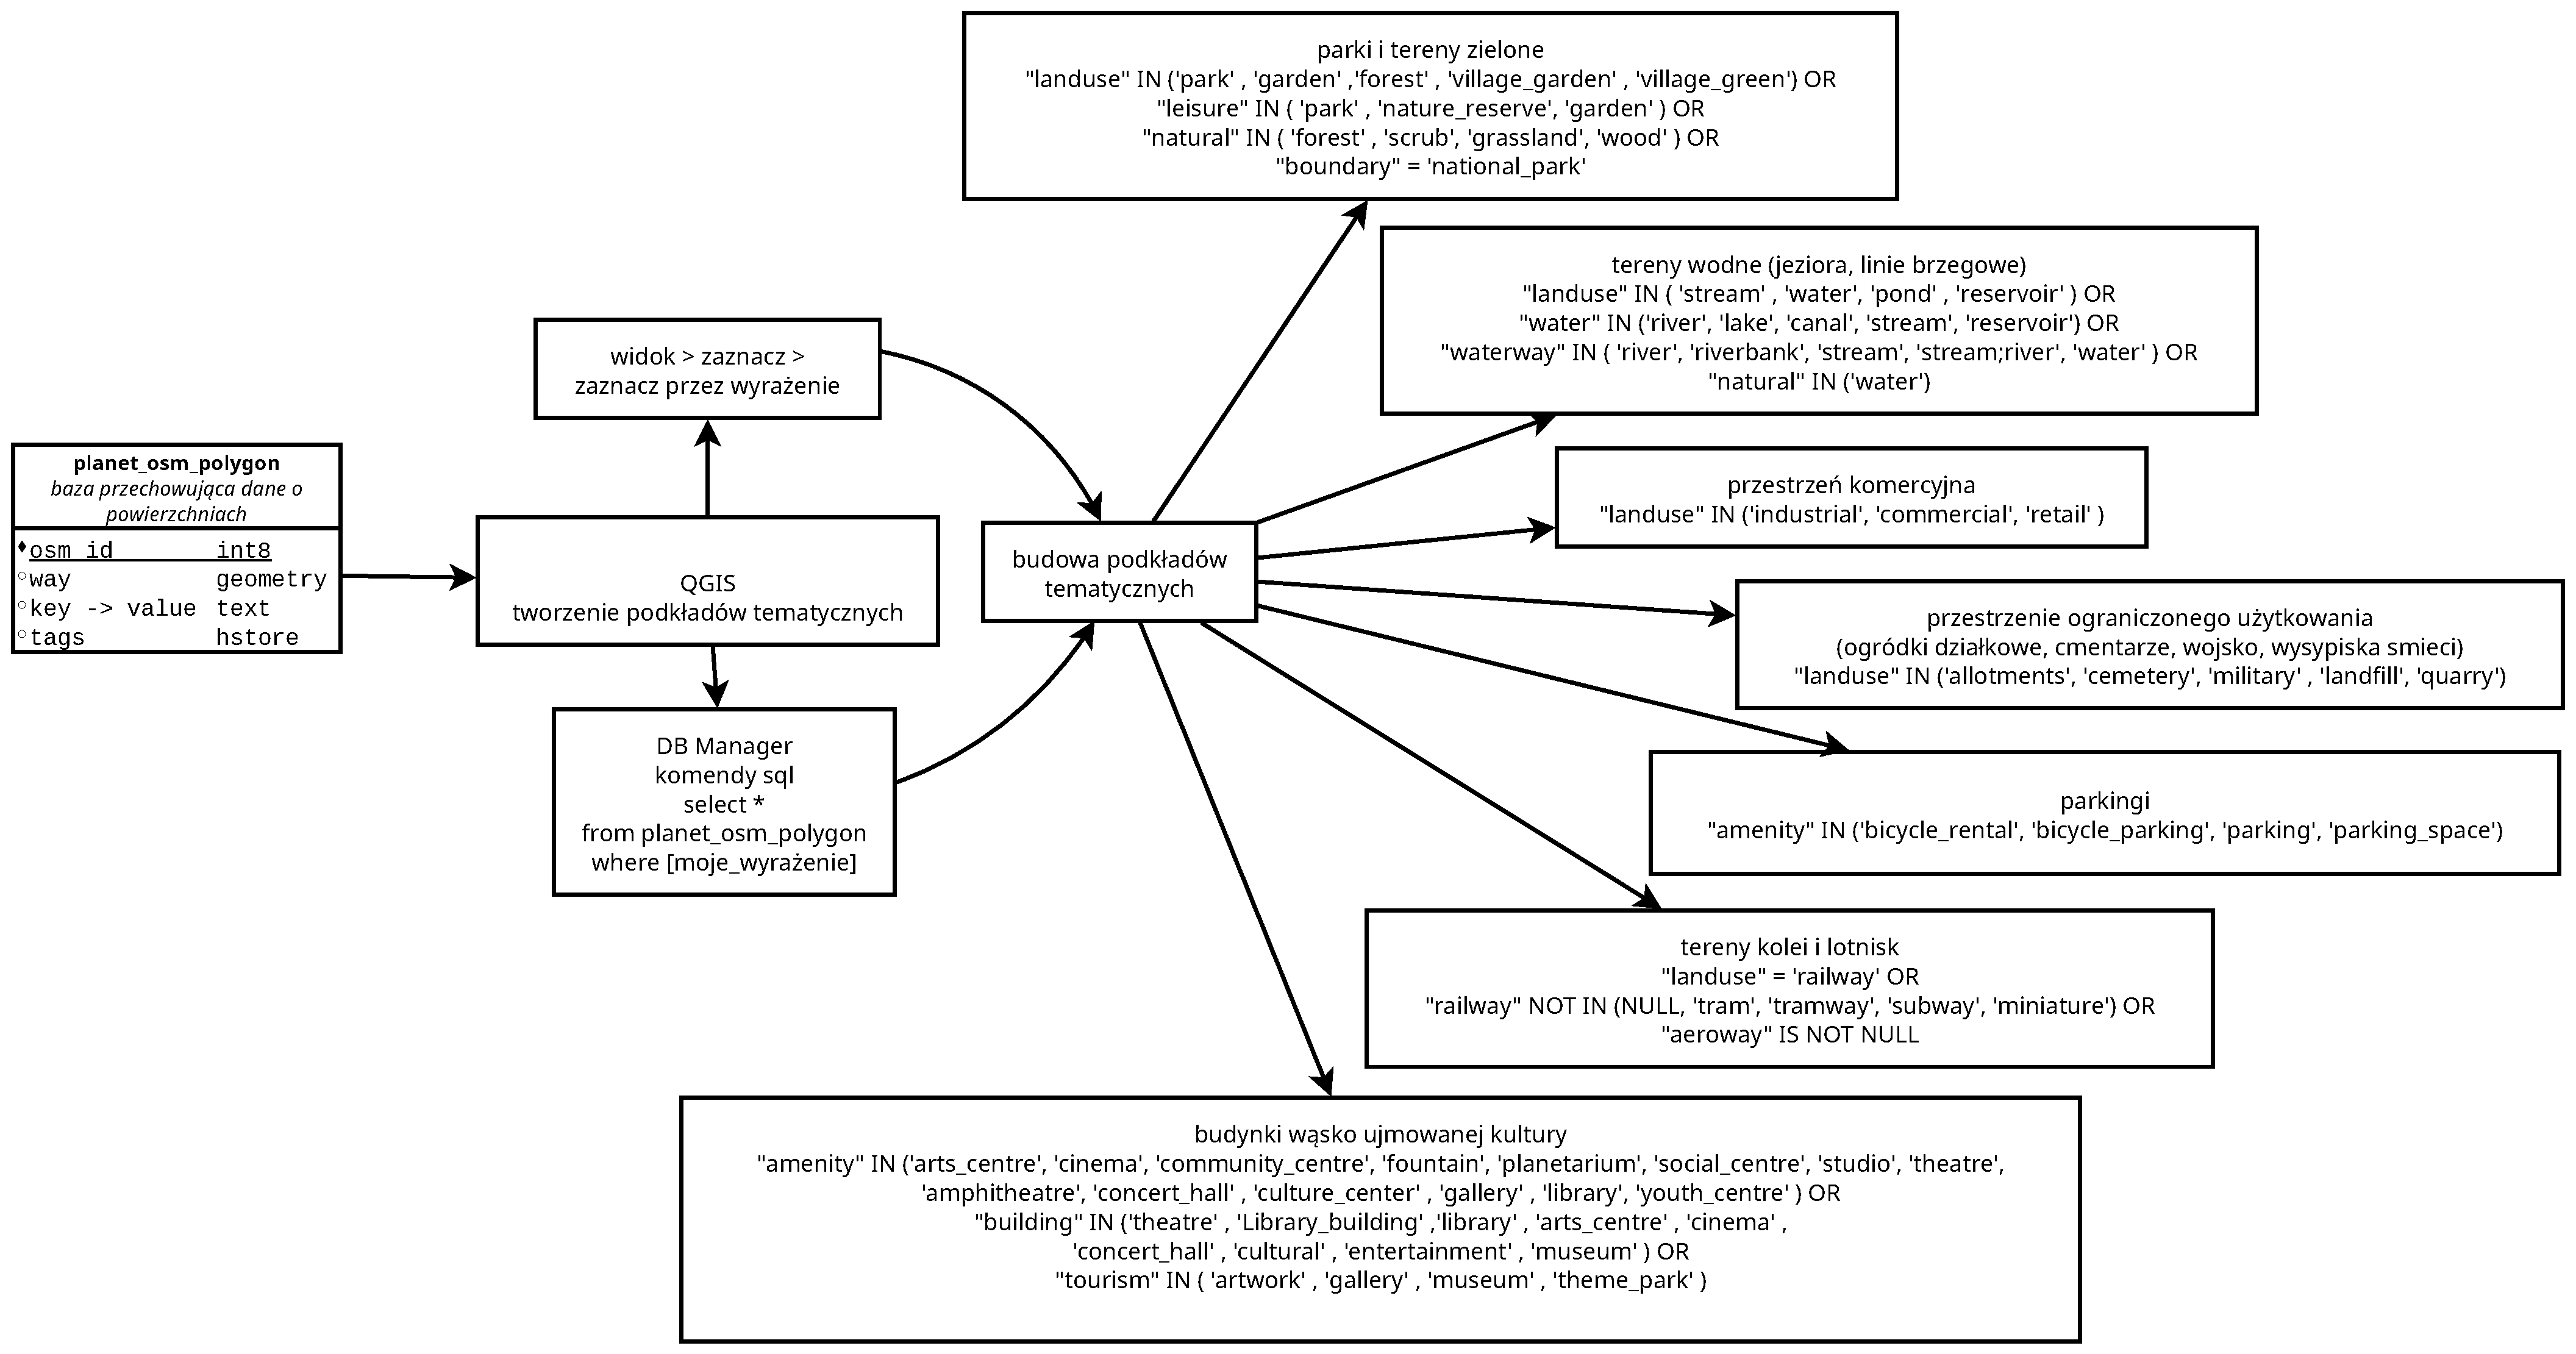
\includegraphics[width=1.5\textwidth]{/Users/mariusz/DokumentyLatex/obrazylatex/schematygislatex/obraz4a.eps}
	
\label{}

\end{figure}
\end{landscape}

\section{Przetwarzanie danych liniowych.}

Sieć drogowa została wygenerowana wg następujących parametrów:
\begin{lstlisting}[ language=SQL, caption={Wybieranie sieci drogowej}]
select * 
from planet_osm_line
where osm_id > 0 AND 
highway IN ('footway' , 'motorway' , 'motorway_link' , 'primary', 'primary_link' , 'residential' , 'residential_link' , 'secondary' , 'secondary_link' , 'tertiary' , 'tertiary_link' , 'trunk' , 'trunk_link' , 'service', 'living_street',  'pedestrian'  )
\end{lstlisting}

Informacje o komunikacji publicznej traktowane są jako relacje, posiadają wartość osm_id mniejszą od 0. Dane te zostały pobrane w następujący sposób:
\begin{lstlisting}[ language=SQL]
select * 
from planet_osm_line
where osm_id  < 0 AND route  IN ( 'trolleybus', 'train','tracks' ,'track' ,'subway' , 'railway', 'bus', 'tram')
\end{lstlisting}

Część informacji o rzekach znajduje się w tabeli z informacjami o liniach:
\begin{lstlisting}[ language=SQL, caption={Wybieranie terenów wodnych.}]
select * 
from planet_osm_line
where (landuse IN ( 'stream' , 'water', 'pond' , 'reservoir' ) OR 
water IN ('river', 'lake', 'canal', 'stream', 'reservoir') OR 
waterway IN ( 'river', 'riverbank', 'stream', 'stream;river', 'water' ) OR 
planet_osm_line.natural IN ('water'))
\end{lstlisting}
\begin{landscape}
	\begin{figure}[htp]
		\caption{Schemat przetwarzania informacji o liniach.}
	\centering
	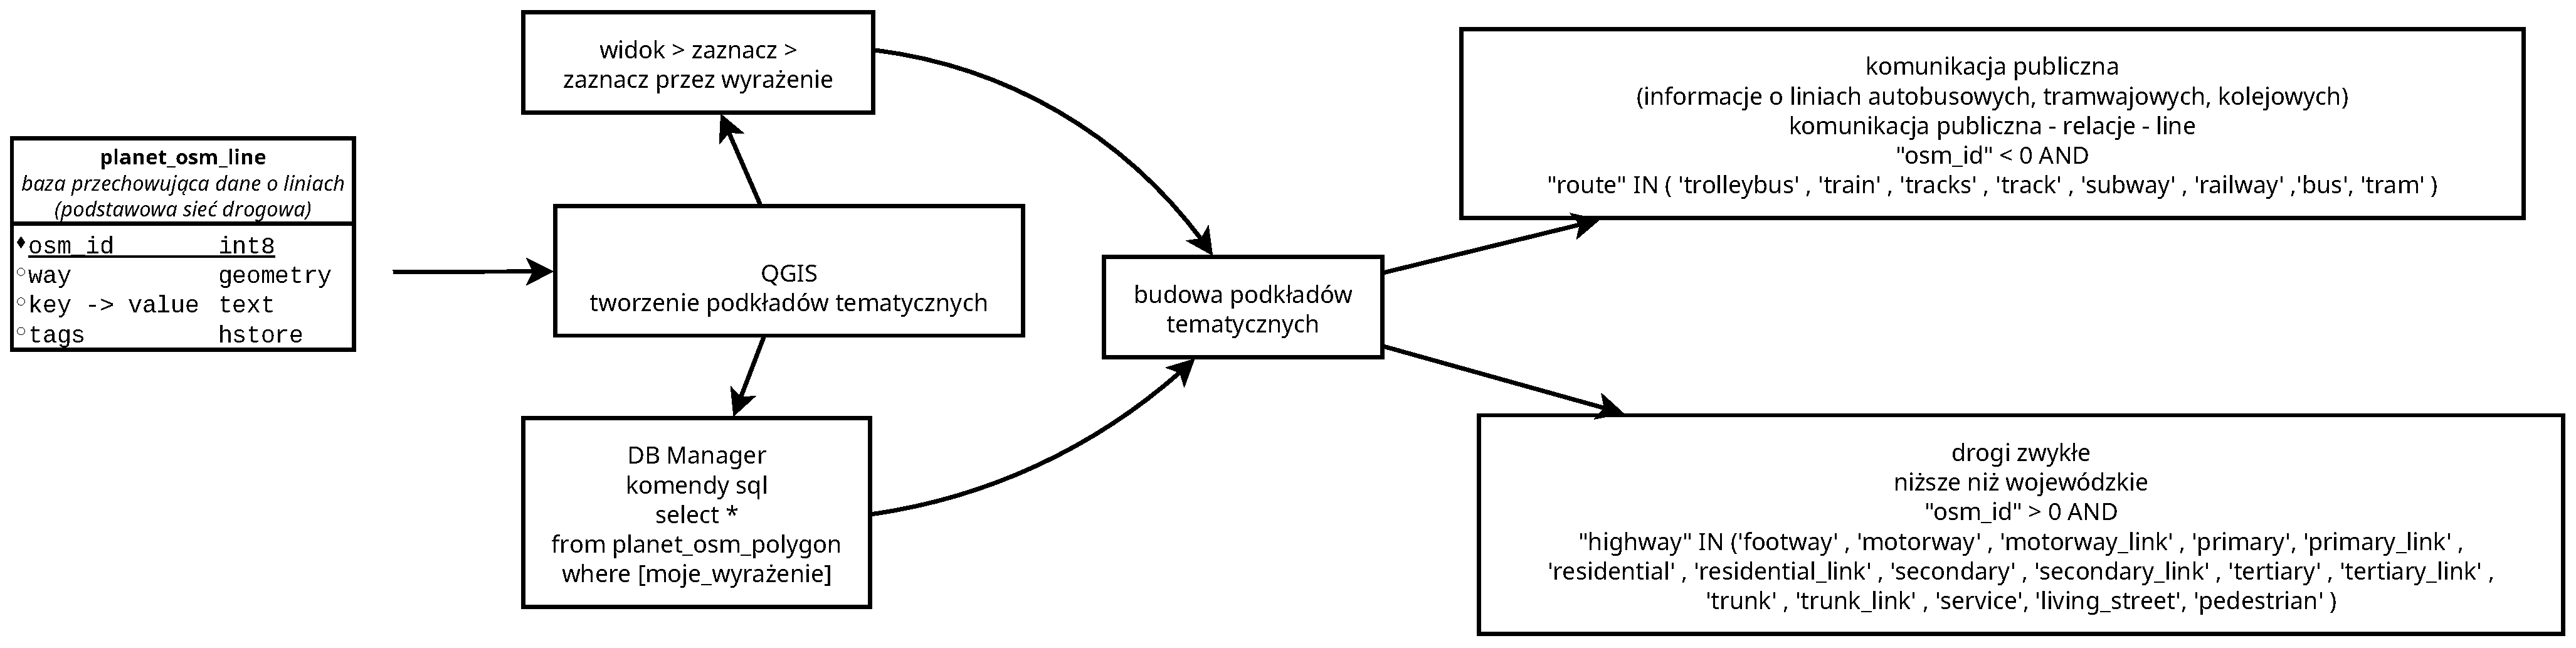
\includegraphics[width=1.6\textwidth]{/Users/mariusz/DokumentyLatex/obrazylatex/schematygislatex/obraz5a.eps}		
		\label{}	
	\end{figure}
\end{landscape}

\section{Przetwarzanie danych o punktach. Dodatek.}

Dane o przystankach znajdują się danych o POI generowanych w oparciu o program osm2poi, jednak algorytm przetwarzania danych nie gromadzi wszystkich obiektów. 
W tym celu z bazy planet_osm_point należy wybrać dodatkowe obiekty
\begin{lstlisting}[ language=SQL, caption={Wybieranie przystanków autobusowych}]
Select *
from planet_osm_point
where 'highway' ILIKE 'bus_stop'
\end{lstlisting}
%%%%%%%%%%%%%%%%
% PQROUTING %
%%%%%%%%%%%%%%%%
\paragraph{Bazy danych.}
W bazie \textit{ozk-gis} znajdują się następujące tabele. Są one pogrupowane w trzech schematach:. 
\begin{itemize}
	\item bazy - dane GUS i inne źródła danych o natężeniu zjawisk
	\item postgres - baza przejściowa
	\item public - dane przestrzenne i słownikowe 
\end{itemize}
\begin{footnotesize}
	\begin{longtable}{p{1.5cm} p{10.2cm}}
		\hline
		\multicolumn{2}{c}{Początek Tabeli}\\
		
		Schemat                        & Nazwa tabeli\\
		\hline
		\endfirsthead
		
		\hline
		\multicolumn{2}{c}{Ciąg dalszy Tabeli}\\
		
		Schemat                        & Nazwa tabeli\\
		\hline
		\endhead
		
		\hline
		\endfoot
		
		\hline
		\multicolumn{2}{ c }{Koniec Tabeli}\\
		\hline\hline
		\endlastfoot
		bazy     & biblioteki\_2015\_gus                                               \\
		bazy     & dojazdy\_praca\_nsp\_2011                                           \\
		bazy     & domy\_kultury\_2015                                                 \\
		bazy     & kina\_2015                                                          \\
		bazy     & licea\_o\_wskazniki\_2015                                           \\
		bazy     & ludnosc\_wg\_lat                                                    \\
		bazy     & muzea\_2015\_gus                                                    \\
		bazy     & szkoly\_ibe                                                         \\
		bazy     & teatry\_2014\_it                                                    \\
		bazy     & wyd\_kult\_gminy                                                    \\
		bazy     & wyd\_kult\_gminy\_1osoba                                            \\
		bazy     & zmiany\_teryt\_gminy                                                \\
		bazy     & zmiany\_teryt\_powiaty                                              \\
		postgres & dochody\_gmin\_2015\_gus                                            \\
		postgres & wydatki\_gmin\_2015\_gus                                            \\
		public   & area\_admin\_level\_8\_osm\_11\_2016                                \\
		public   & area\_dzialki\_cemntarze\_osm\_20\_10\_2016                         \\
		public   & area\_koleje\_osm\_20\_10\_2016                                     \\
		public   & area\_kultura\_osm\_20\_10\_2016                                    \\
		public   & area\_medycyna\_osm\_20\_10\_2016                                   \\
		public   & area\_parkingi\_komunikacja\_osm\_20\_10\_2016                      \\
		public   & area\_parki\_osm\_20\_10\_2016                                      \\
		public   & area\_parki\_osm\_5\_11\_2016                                       \\
		public   & area\_przemysl\_handel\_osm\_20\_10\_2016                           \\
		public   & area\_publiczne\_straz\_policja\_osm\_20\_10\_2016                  \\
		public   & area\_religijne\_osm\_20\_10\_2016                                  \\
		public   & area\_rodzaje\_powierzchni\_rolnicze\_mieszkalne\_osm\_20\_10\_2016 \\
		public   & area\_sport\_osm\_20\_10\_2016                                      \\
		public   & area\_szkolnictwo\_osm\_20\_10\_2016                                \\
		public   & area\_zabudowa\_komercyjna\_20\_10\_2016                            \\
		public   & biblioteki\_mkidn\_2014                                             \\
		public   & biblioteki\_wroclaw\_open                                           \\
		public   & domy\_kultury\_2014                                                 \\
		public   & drogi\_bdoo\_2016                                                   \\
		public   & drogi\_glowne\_osm\_15\_11\_2016\_obsolete                          \\
		public   & drogi\_zwykle\_osm\_18\_11\_2016                                    \\
		public   & gminy                                                               \\
		public   & gminy\_historyczne                                                  \\
		public   & gminy\_osm\_teryt                                                   \\
		public   & komunikacja-lotniska                                                \\
		public   & kopalnie\_bdoo\_06\_2016                                            \\
		public   & krs\_2016                                                           \\
		public   & krs\_ost                                                            \\
		public   & layer\_styles                                                       \\
		public   & linie\_relacje\_komunikacja\_publiczna\_osm\_5\_11\_2016            \\
		public   & ludnosc\_NSP2011                                                    \\
		public   & miejscowosci                                                        \\
		public   & obreby\_ewidencyjne                                                 \\
		public   & obszar\_natura\_2000\_bdoo\_2016                                    \\
		public   & obwod spisowy                                                       \\
		public   & osm\_poi\_15\_11\_2016                                              \\
		public   & osm\_poi\_17\_12\_2016                                              \\
		public   & osm\_poi\_custom\_acces\_15\_11\_2016                               \\
		public   & osm\_poi\_custom\_acces\_30\_10\_2016                               \\
		public   & osm\_poi\_przystanki\_acces\_20\_10\_2016                           \\
		public   & osm\_poi\_przystanki\_\_bus\_20\_10\_2016                           \\
		public   & otwartezabytki\_09\_10\_2016                                        \\
		public   & park\_krajobrazowy\_bdoo\_2016                                      \\
		public   & park\_narodowy\_bdoo\_2016                                          \\
		public   & people\_km2\_NSP                                                    \\
		public   & powiaty                                                             \\
		public   & rejony statystyczne                                                 \\
		public   & rezerwaty\_bdoo\_06\_2016                                           \\
		public   & siec\_kolejowa\_bdoo\_2016                                          \\
		public   & slownik\_indeksy\_ozk                                               \\
		public   & slownik\_osm\_28\_11\_2016                                          \\
		public   & slownik\_ozk\_28\_11\_2016                                          \\
		public   & spatial\_ref\_sys                                                   \\
		public   & teatry\_danewarszawskie                                             \\
		public   & temp\_krs\_99                                                       \\
		public   & wody\_ladowe\_osm\_20\_10\_2016                                     \\
		public   & wody\_ladowe\_powierz\_5\_11\_2016                                  \\
		public   & wojewodztwa                                             		
		
	\end{longtable}
\end{footnotesize}	

\begin{lstlisting}[language=SQL,caption={Nazwy tabel z bazy.}]
select * from information_schema.tables
where table_schema IN ('public', 'postgres','bazy') and table_type not like 'VIEW'
order by table_schema, table_name
\end{lstlisting}
\begin{lstlisting}[language=SQL,caption={Liczebności obiektów w gminach ze względu na typ(funkcja grupująca).}]
select count(ozk_indeks_id)as liczba, 
ozk_indeks_id,count(forma_prawna_str) as liczba_obiektow_krs, 
forma_prawna_str,slownik_ozk_28_11_2016.nazwa,gminy.jpt_nazwa_, gminy.jpt_kod_je
from krs_2016
left join  slownik_ozk_28_11_2016 
on krs_2016.ozk_indeks_id = slownik_ozk_28_11_2016.id 
inner join gminy
on st_intersects(gminy.geom, krs_2016.geom)
group by ozk_indeks_id, forma_prawna_str,slownik_ozk_28_11_2016.nazwa,gminy.jpt_nazwa_,gminy.jpt_kod_je
order by gminy.jpt_kod_je,gminy.jpt_nazwa_, ozk_indeks_id,liczba, forma_prawna_str
\end{lstlisting}

\chapter{Podstawowe operacje w SQL}		

\begin{lstlisting}[language=SQL, caption={Łaczenie gmin z danymi GUS.}]
Select gminy.geom, bazy.wyd_kult_gminy.*
from bazy.wyd_kult_gminy 
left join gminy
on bazy.wyd_kult_gminy.kod::integer = gminy.jpt_kod_je::integer
/*rzutowanie typu*/
\end{lstlisting}

\begin{lstlisting}[language=SQL, caption={Operacje matematyczne.}]
select gminy_osm_teryt.teryt, way, ("2015"::integer) - ("2005"::integer) as zmian_liczebnosc
from ludnosc_wg_lat
left join gminy_osm_teryt
on  ludnosc_wg_lat.teryt = gminy_osm_teryt.teryt
order by zmian_liczebnosc
\end{lstlisting}

\begin{lstlisting}[language=SQL, caption={Export danych do csv.}]
COPY
(SELECT <ZAPYTANIE>) 
TO plik.csv CSV DELIMITER ','
/*plik zapisuje się w katalogu tmp*/
\end{lstlisting}
\chapter{Portret gminy}

Wyodrębnienie obiektów z gminy:
\begin{lstlisting}[language=SQL, caption={Obiekty z gminy.}]
Select osm.geom, osm.id, osm.nazwa, gminy.jpt_nazwa_, osm.kod_osm, osm.slownik_osm_713_nazwa_osm	
from osm_poi_custom_acces_5_11_2016 as osm
/*wewnętrzne złączenie z obiektami, które się przecinają */
Inner join public.gminy as gminy on st_intersects(osm.geom, gminy.geom)
/*wyszukanie gminy po kodzie teryt, wyodrębnienie tagu */
where gminy.jpt_kod_je ILIKE '2805011' and osm.slownik_osm_713_nazwa_osm not ILIKE '%place%'
group by slownik_osm_713_nazwa_osm, osm.geom, osm.id, osm.nazwa, gminy.jpt_nazwa_
\end{lstlisting}

Wyodrębnienie informacji o zagęszczeniu ludności w gminie:
\begin{lstlisting}[language=SQL,caption={Ludność w gminie na km$^{2}$.}]
SELECT ST_Intersection(osm.geom, gminy.geom), osm.value
from public."ludnosc_NSP2011" as osm, public.gminy as gminy
where st_intersects(osm.geom, gminy.geom) and gminy.jpt_kod_je ILIKE '2805022'
group by value, osm.id, osm.geom, gminy.geom
\end{lstlisting}
Typy obiektów OZK:
\begin{lstlisting}[language=SQL,caption={Typy obiketów OZK.}]
SELECT slownik_osm_713_nazwa_osm,
COUNT(DISTINCT osm_poi_custom_acces_5_11_2016.id) As tot
/* wczytaj obiekty z kolumny slownik_osm_709 zlicz je wg kolumnu id(dla odrębnych wartości) i pokaż kolumnę jako tot
*/
FROM public.osm_poi_custom_acces_5_11_2016
INNER JOIN public.gminy As g
ON ST_Within(osm_poi_custom_acces_5_11_2016.geom, g.geom)
/* zrób złaczenie przestrzenne z baza gmin (nazywaj jako g) -
złączenie według kolumn z geometrialmi przestrzennymi
*/
WHERE g.jpt_kod_je = '1201011'  AND osm_poi_custom_acces_5_11_2016.slownik_osm_713_nazwa_osm NOT ILIKE '%place%'
/* wybierz kolumnę z nazwa z gminy i znajdź tam Bolesławiec
*/
GROUP BY public.osm_poi_custom_acces_5_11_2016.slownik_osm_713_nazwa_osm
/* grupuj wg kolumny wybranej na samym początku po select
*/
ORDER BY tot DESC;
\end{lstlisting}
Obiekty w buforze 1 km od punktu
\begin{lstlisting}[language=SQL,caption={Obieky w okolicy 1km od obiektu z osm}]
SELECT ROW_NUMBER() OVER (
PARTITION BY loc.osm_id
ORDER BY st_distance(r.geom, loc.geom), r.nazwa) As row_num,	
loc.nazwa, loc.id, loc.slownik_osm_713_nazwa_osm, 
loc.geom, loc.wheelchair, loc.url, loc.weebsite, loc.opening_hours,
st_distance(r.geom, loc.geom) as dist_m
FROM osm_poi_custom_acces_5_11_2016 as loc
LEFT JOIN osm_poi_przystanki_acces_20_10_2016 as r 
ON st_dwithin(r.geom, loc.geom, 1000)
/* buffor 1000m*/
WHERE loc.slownik_osm_713_nazwa_osm IS NOT NULL AND loc.nazwa IS NOT NULL AND r.osm_id ILIKE '%N48267476%' AND loc.slownik_osm_713_nazwa_osm NOT ilike '%place%'
\* N48267476 (przykładowy kod obiektu) wyznaczany wg kodu obiektu z bazy osm z programu osm2poi
GROUP BY r.geom, loc.geom, loc.nazwa, r.nazwa, loc.id, loc.slownik_osm_713_nazwa_osm, loc.wheelchair, loc.url, loc.weebsite, loc.opening_hours
ORDER BY dist_m, r.nazwa, row_num
\end{lstlisting}
Typy obiektów osm - zliczenie
\begin{lstlisting}[language=SQL,caption={Typy obiektów osm - zliczenie}]
SELECT 
slownik_osm_713_nazwa_osm,
COUNT(DISTINCT osm_poi_custom_acces_5_11_2016.id) As tot
/* wczytaj obiekty z kolumny slownik_osm_709 zlicz je wg kolumnu id(dla odrębnych wartości) i pokaż kolumnę jako tot
*/
FROM 
public.osm_poi_custom_acces_5_11_2016
INNER JOIN public.gminy As g
ON ST_Within(osm_poi_custom_acces_5_11_2016.geom, g.geom)
/* zrób złaczenie przestrzenne z baza gmin (nazywaj jako g) - złączenie według kolumn z geometrialmi przestrzennymi
*/
WHERE g.jpt_kod_je = '1201011'  AND osm_poi_custom_acces_5_11_2016.slownik_osm_713_nazwa_osm NOT ILIKE '%place%'
/* wybierz kolumnę z nazwa z gminy i znajdź tam Bolesławiec
*/
GROUP BY public.osm_poi_custom_acces_5_11_2016.slownik_osm_713_nazwa_osm
/* grupuj wg kolumny wybranej na samym początku po select
*/
ORDER BY tot DESC;
\end{lstlisting}
Tworzenie buffora.
\begin{lstlisting}[language=SQL,caption={Buffor 1km}]
select id, nazwa, 
st_buffer(geom,1000) as buffer_1000
from osm_poi_custom_acces_5_11_2016 as osm
/*nazwa obiektu z bazy osm - po kodzie id*/
where osm.id = 29635
\end{lstlisting}
\begin{lstlisting}[language=SQL,caption={Obiekty wokół 1km od koordynatów geograficznych}]
select *
from krs
Where st_dwithin(geom,
/* przekształć układ z 4326 */
ST_Transform(
/* ustaw układ na 2180 */
ST_SetSRID(ST_Point(17.031924, 51.109566 ), 4326), 2180), 1000)
\end{lstlisting}

Możliwe jest także wyliczanie długości dróg w gminie ( czy też z polygonów). W tym celu należy znaleźć odpowiednie id polygonu i następnie odpytać bazę danych osm.
\begin{lstlisting}[language=SQL,caption={Znalezienie id polygonu}]
SELECT osm_id FROM planet_osm_polygon
WHERE boundary='administrative' AND admin_level='7' AND name='Warszawa';
\end{lstlisting}
Krok kolejny to znalezienie długości dróg pierwszego rzędu (autostrad i dróg ekspresowych)
\begin{lstlisting}[language=SQL,caption={Długość dróg w polygonie według osm_roads}]
SELECT
round(SUM(
ST_Length(ST_Transform(
ST_Intersection(way, (SELECT way FROM planet_osm_polygon WHERE osm_id=-2907540))
,4326)::geography)
)) AS "distance (meters)", highway AS "highway type"
FROM planet_osm_roads
WHERE highway IS NOT NULL
AND ST_Intersects(way, (SELECT way FROM planet_osm_polygon WHERE osm_id=-2907540))
GROUP BY highway
ORDER BY "distance (meters)" DESC
LIMIT 10;
\end{lstlisting}
Następnie należy wyliczyć pozostałe drogi z osm_line
\begin{lstlisting}[language=SQL,caption={Długość dróg w polygonie według osm_lines}]
SELECT
round(SUM(
ST_Length(ST_Transform(
ST_Intersection(way, (SELECT way FROM planet_osm_polygon WHERE osm_id=-2907540))
,4326)::geography)
)) AS "distance (meters)", highway AS "highway type"
FROM planet_osm_line
WHERE highway IS NOT NULL
AND ST_Intersects(way, (SELECT way FROM planet_osm_polygon WHERE osm_id=-2907540))
GROUP BY highway
ORDER BY "distance (meters)" DESC
LIMIT 10;
\end{lstlisting}

\chapter{Izochron}



\begin{lstlisting}[language=SQL,caption={Tworzenie izochronu }]

CREATE TABLE hh_2po_4pgr_node_59980_1_km AS
SELECT * FROM hh_2po_4pgr_nodes
JOIN
(SELECT * FROM pgr_drivingDistance('
SELECT id AS id,
source::int4 AS source,
target::int4 AS target,
-- koszty podróży z kolmny km
km::float8 AS cost
FROM hh_2po_4pgr',
-- id węzła od którego wyliczany jest isochron
59980,
-- odległość 
1,
false,
false)) AS hh_2po_4pgr_nodes_cost
ON
hh_2po_4pgr_nodes.id = hh_2po_4pgr_nodes_cost.id1
;
\end{lstlisting}

\begin{lstlisting}[language=SQL,caption={Tworzenie izochronu 2}]
Drop table hh_2po_4pgr_node_59980_1_ok_km;
-- tworzenie isochronu
CREATE TABLE hh_2po_4pgr_node_59980_1_ok_km AS
SELECT * FROM hh_2po_4pgr_nodes
JOIN
(SELECT * FROM pgr_drivingDistance('
SELECT id AS id,
source::int4 AS source,
target::int4 AS target,
-- koszty podróży z kolmny km
km::float8 AS cost
FROM hh_2po_4pgr',
-- id węzła od którego wyliczany jest isochron
393690,
-- odległość 
1,
false,
false)) AS hh_2po_4pgr_nodes_cost
ON
hh_2po_4pgr_nodes.id = hh_2po_4pgr_nodes_cost.id1
;
\end{lstlisting}
\begin{lstlisting}[language=SQL,caption={Otoczka wypukła}]

SELECT 
st_convexhull(ST_Collect(geom_way))
FROM hh_2po_4pgr_node_59980_1_ok_km;
\end{lstlisting}

\begin{landscape}
	\begin{figure}[htp]
		\caption{Schemat tworzenie izochronu.}
		\centerline{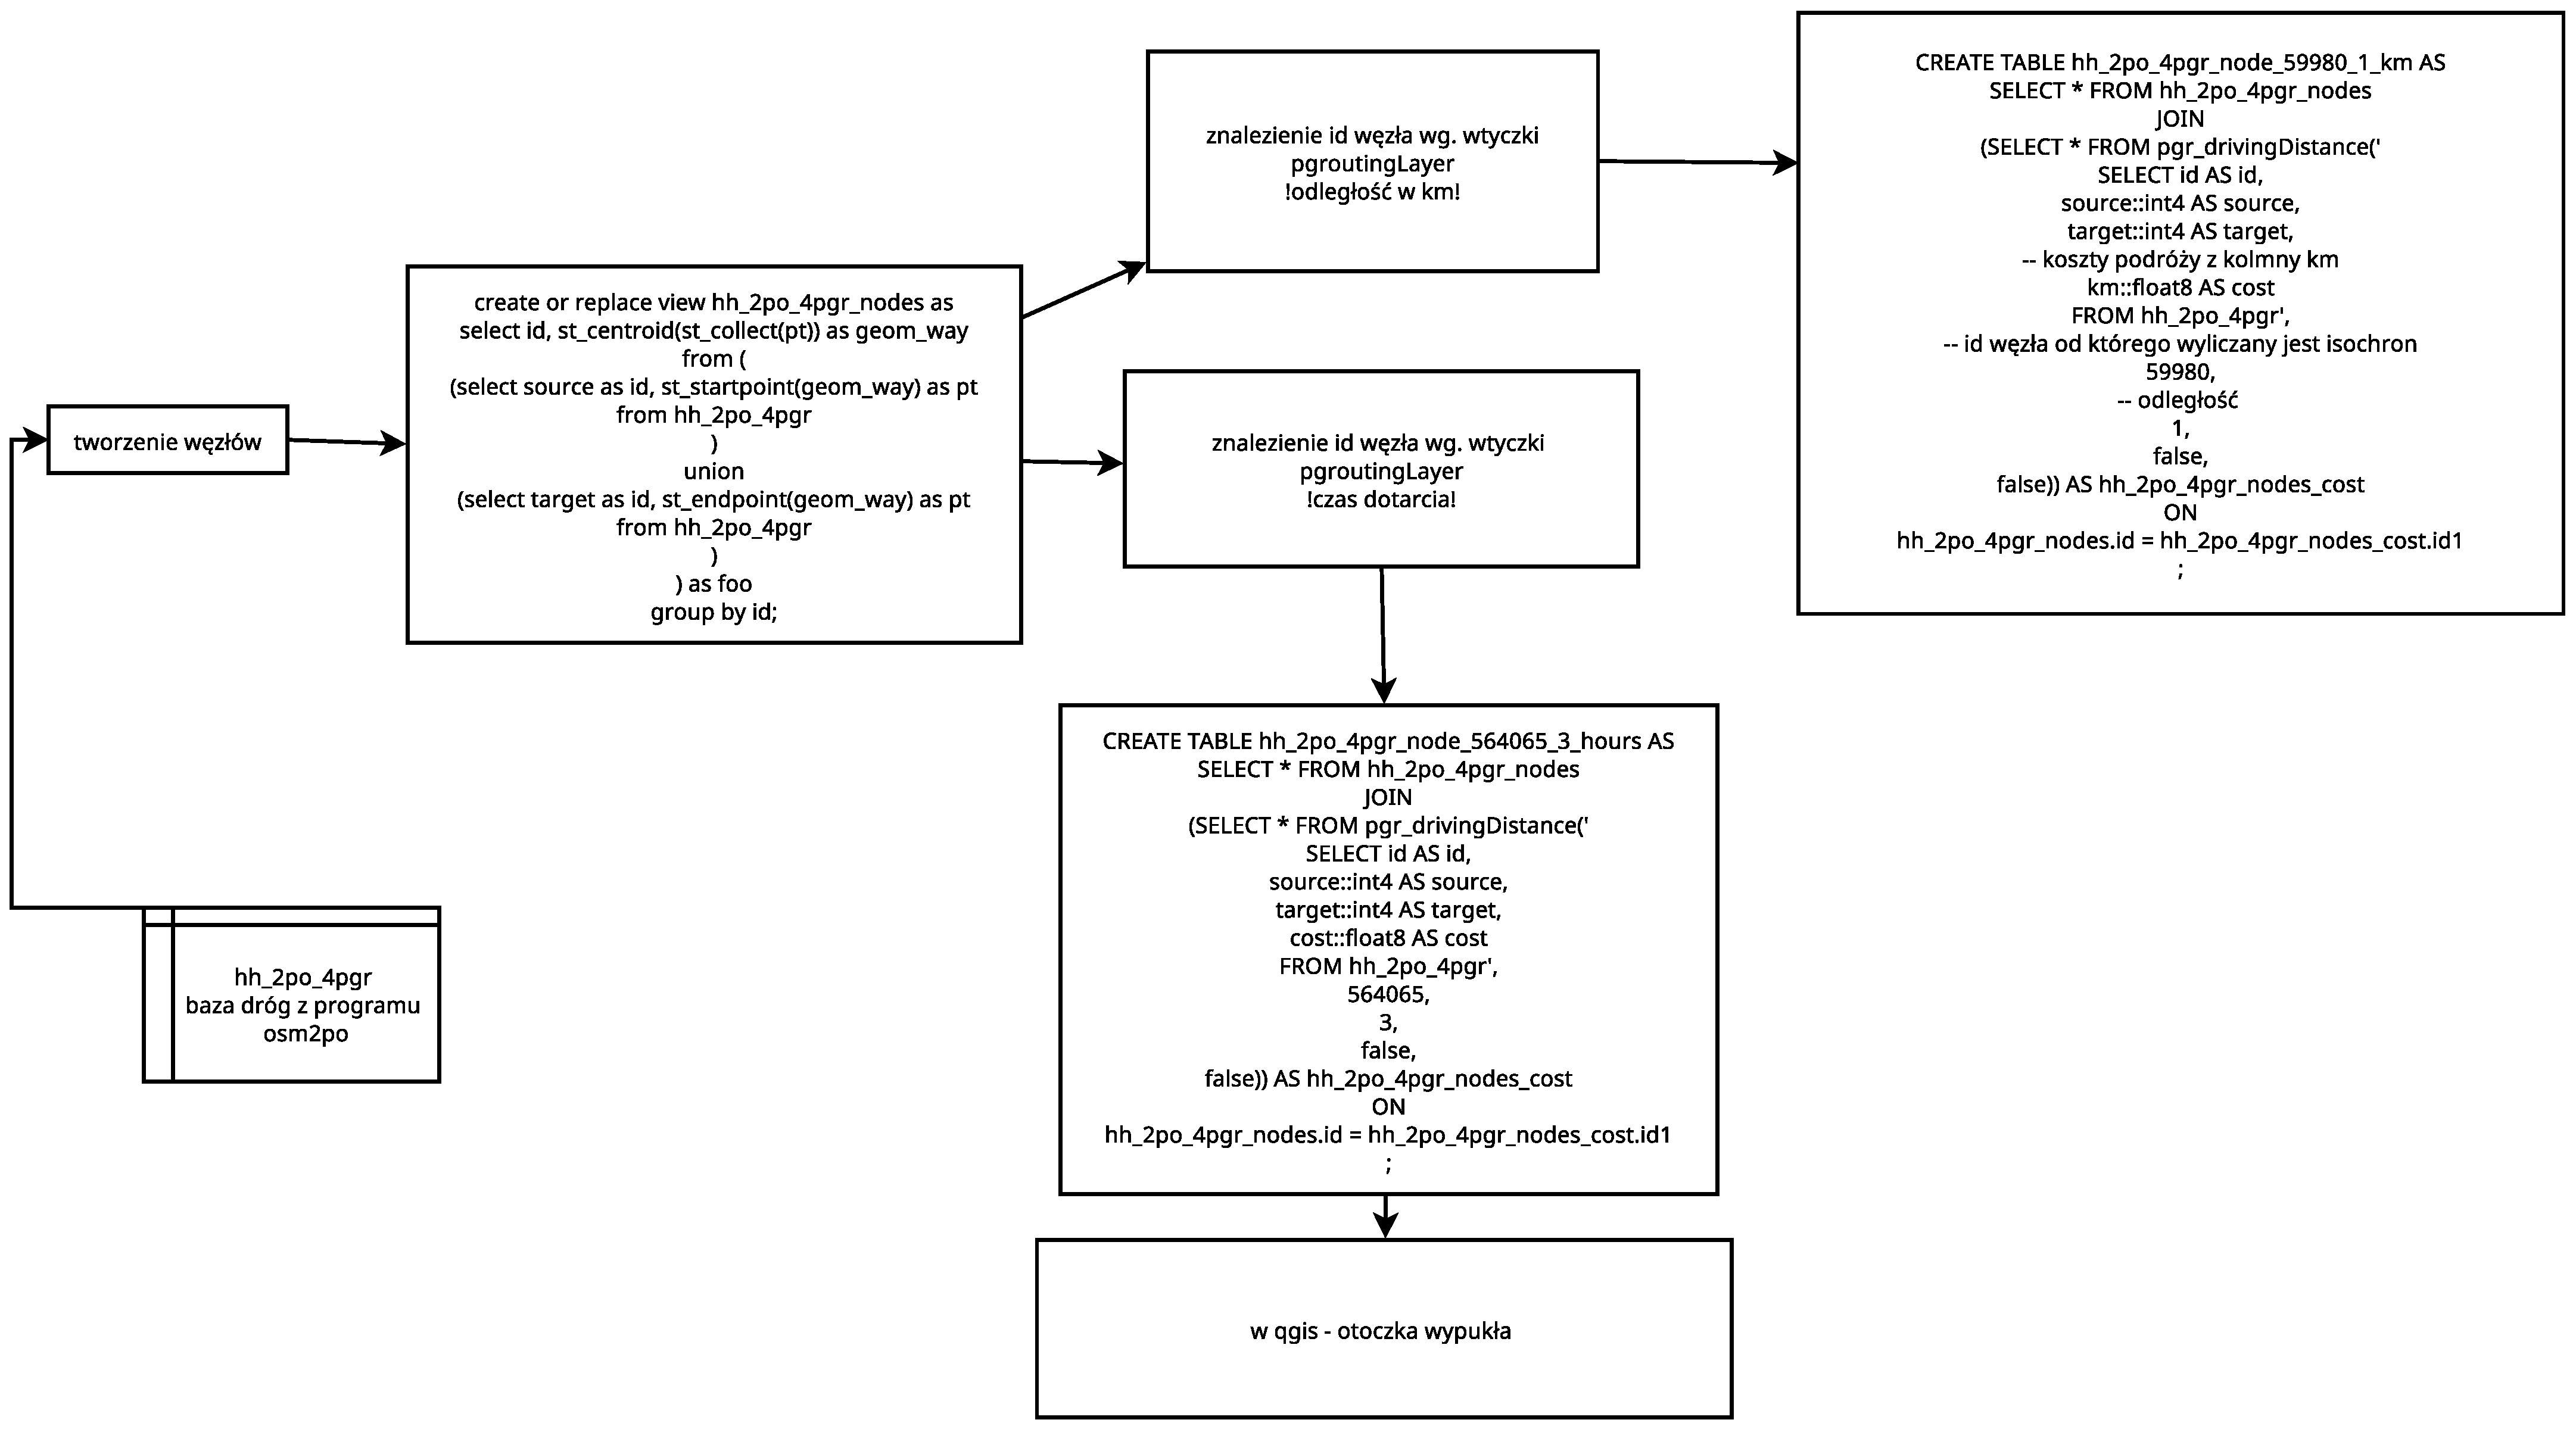
\includegraphics[width=26.5cm]{/Users/mariusz/DokumentyLatex/obrazylatex/schematygislatex/isochrony.eps}}
		\label{}
		
	\end{figure}
\end{landscape}

\chapter{Podstawowe komendy postgis}

\begin{itemize}
	\item \textbf{st_buffer}(<geometrie - projekcja 2180>,<odległość w metrach>) - tworzenie buffora;
	
	\item\textbf{st_intersects}(<geometrie danych A - projekcja 2180>,<geometrie danych B - projekcja 2180>) - powierzchnie przecinające 
\end{itemize}


\chapter{Rozwiązania częstych problemów składni SQL.}
\section{Bazy oparte o kod systemu TERYT.}
\subsection{\textit{Leading zero.}}

Bazy, które opierają się przy identyfikacji gmin na kodach teryt mogą sprawiać problemy przy imporcie do systemu postgres. System Teryt jest 7 cyfrowy, natomiast 4 województwa mają kod z zakresu 02, 04, 06, 08. W trakcie importu do baz danych "wiodące zero" (\textit{leading zero}) jest pomijane.\\
 \textbf{Przetwarzanie danych w locie.} Kiedy odwołania wg gmin są po kodach teryt można połączyć je (JOIN) dodając w zapytaniu komendę
	\begin{lstlisting}[ language=SQL]
	lpad(<kolumna_z_kodem_teryt>,7,'0')::text
	\end{lstlisting}
\subsection{Funkcje warunkowe i spajające.}
W sytuacji, kiedy brakuje identyfikatora rodzaju gminy (dane w taki sposób udostępnia IBE)\footnote{\url{http://zpd.ibe.edu.pl/doku.php}}, należy stworzyć nowe kody. W pierwszym kroku - przekształcenie oparte o funkcje warunkową. 

\begin{lstlisting}[ language=SQL]
Select *,
	case when rodzaj_2016 = 'm' then 1
	when rodzaj_2016 = 'w' then 2
	when rodzaj_2016 = 'mw' then 3
	when rodzaj_2016 = 'mnpp' then 1
	end as  typ_numeryczny_gminy
		into zmiany_gminy1
from <baza_danych>;
\end{lstlisting}

Drugim krokiem jest użycie funkcji spajającej kolumny:
\begin{lstlisting}[ language=SQL]
Select *,
	concat(teryt_2016, typ_numeryczny_gminy::varchar)
	as teryt_gminy_2016
	into zmiany_gminy2
from zmiany_gminy1
\end{lstlisting}
\subsection{Przycinanie komórek i wartości w locie.}
Przydatne jest tworzenie złączeń(JOIN) w oparciu o określenie fragmentu ciągu znaków. Przykład na danych o dojazdach do pracy
\begin{lstlisting}[ language=SQL]
select bazy.dojazdy_praca_nsp_2011.*, way
from bazy.dojazdy_praca_nsp_2011
left join gminy_osm_teryt
on left(bazy.dojazdy_praca_nsp_2011.teryt_zamieszk,6) = left(gminy_osm_teryt.teryt,6)
\end{lstlisting}
\subsection{Granice administracyjne.}
W celu wyodrębnienia granic gmin (wraz z kodami teryt) z bazy OSM można użyć następującej komendy:
\begin{lstlisting}[ language=SQL, caption=Gminy z OSM]
select *
into gminy
from planet_osm_polygon
where  admin_level = '7' and  (tags->'teryt:terc' IS not null)
\end{lstlisting}

Wygenerowanie mapy powiatów to zmiana admin_level = '6'

\subsection{Dzielnice Warszawy.}
Wyodrębnienie dzielnic Warszawy polega na wyciągnięciu rekordów admin_level 9 i obszaru z terytami dla woj. mazowieckiego i gminy Warszawa
\begin{lstlisting} [language=SQL, caption=Dzielnice warszawy]
	select *
	from planet_osm_polygon
	where  admin_level = '9'  and (tags->'teryt:terc' ILIKE '%1465%')
\end{lstlisting}


\subsection{Gminy wg zaborów}
Stworzenie aktualnej bazy gmin wg zaborów wymaga wykorzystania pliku z danymi historycznymi i przerobienie go do postaci, w której w jednej kolumnie będą dane o historii. 
\begin{lstlisting} [language=SQL]
Select id, geom, jpt_nazwa_, jpt_kod_je,
case when ziemie_odzyskane = 'T' then 'ziemie odzyskane'
when zabor_austriacki = 'T' then 'zabor austriacki'
when zabor_pruski = 'T' then 'zabor pruski'
when zabor_rosyjski = 'T' then 'zabor rosyjski'
end as  zabor_historyczny
into public.gminy_historyczne_2017
from postgres.gminy_historyczne_2017
\end{lstlisting}
\section{Pozostałe dane.}
\subsection{Tagi przechowywane jako hstore.}

Przekształć hstore w kolumny i dodaj do nowej tabeli: (DO POPRAWKI!!! - hstore w nowych wersjach postgresa tworzy tylko kolumny - key - value.)
\begin{lstlisting}[ language=SQL]
select *, (EACH(tags::hstore) ).*
into gminy_osm_hstore
from gminy_osm
\end{lstlisting}
Alternatywnie należy stworzyć nową bazę danych z komendy wyżej i wybrać tylko
\begin{lstlisting}[ language=SQL]
select *
from gminy_osm_hstore
where gminy_osm_hstore.key = 'teryt:terc'
\end{lstlisting}
tworząc kolejną bazę danych.\\

 W nowej wersji czynność należy zrobić w dwóch krokach. Po po pierwsze należy z bazy planet_osm_polygon wybrać gminy (tak jak jest to przedstawione wcześniej) i wrzucić to do nowej tabeli gminy. Następnie należy stworzyć plik gmin, geometrii oraz nazw i terytów wyodrębnionych z kolumny tags (hstore).
 \begin{lstlisting}[ language=SQL, caption=Teryty jako kolumna - hstore]
 SELECT osm_id, name, way, h->'teryt:terc' AS teryt
 into [gminy_osm_rok]
 FROM  (SELECT osm_id,name, way, tags AS h FROM [gminy]) t;
 
\end{lstlisting}
\subsection{Rzutowanie typu.}
Postgres "nie lubi" nazw kolumn, które są całkowicie liczbowe. Jednak można zmusić system do wykonywania operacji. Przykład na danych GUS:
\begin{lstlisting}[ language=SQL]
select region, teryt, ("2015"::integer) - ("2005"::integer)
		 as zmian_liczebnosc
from ludnosc_wg_lat
order by zmian_liczebnosc
\end{lstlisting}

\chapter{Analiza i wizualizacja danych w programie QGIS.}

Prezentowane porady dotyczą wersji 3.6.x, która stanowi wersję LTR, czyli nie pojawiają się w niej nowe funkcjonalności, a jedynie poprawki błędów. 
W systemie macos należy wcześniej zainstalować pakiet Python w wersji 3.6 (w czerwcu 2019 była to wersja 3.6.8), jest on dystrybuowany osobno. W systemie Linux jest to zależne od dystrybucji. Arch ma w chwili obecnej pakiet zbudowany, do pobrania menadżerem pacman. Wersja dla Windows posiada instalator sieciowy, który zajmuje się pobraniem i zainstalowaniem niezbędnych dodatków i zależności. 
\section{Wczytywanie danych.}

\subsection{Edycja plików DBF dla QGIS}

Pliki shp składają się z pięciu elementów, jednym są dane zawarte w pliku dbf, w którym są zapisane wartości dla atrybutów. Plik można otworzyć w arkuszu kalkulacyjnym. Jednak, aby zachować strukturę plików, należy zapisując pamiętać o dokładnie takiej samej kolejności w pliku. 


\appendix
\chapter{default.style}
	
	\begin{verbatim}
	# This is the default osm2pgsql .style file that comes with osm2pgsql.
	#
	# A .style file has 4 columns that define how OSM objects end up in tables in
	# the database and what columns are created. It interacts with the command-line
	# hstore options.
	#
	# Columns
	# =======
	#
	# OsmType: This is either "node", "way" or "node,way" and indicates if this tag
	# applies to nodes, ways, or both.
	#
	# Tag: The tag
	#
	# DataType: The type of the column to be created. Normally "text"
	#
	# Flags: Flags that indicate what table the OSM object is moved into.
	#
	# There are 6 possible flags. These flags are used both to indicate if a column
	# should be created, and if ways with the tag are assumed to be areas. The area
	# assumptions can be overridden with an area=yes/no tag
	#
	# polygon - Create a column for this tag, and objects with the tag are areas
	#
	# linear - Create a column for this tag
	#
	# nocolumn - Override the above and don't create a column for the tag, but do
	# include objects with this tag
	#
	# phstore - Same as polygon,nocolumn for backward compatibility
	#
	# delete - Drop this tag completely and don't create a column for it. This also
	# prevents the tag from being added to hstore columns
	#
	# nocache - Deprecated and does nothing
	#
	# If an object has a tag that indicates it is an area or has area=yes/1,
	# osm2pgsql will try to turn it into an area. If it succeeds, it places it in
	# the polygon table. If it fails (e.g. not a closed way) it places it in the
	# line table.
	#
	# Nodes are never placed into the polygon or line table and are always placed in
	# the point table.
	#
	# Hstore
	# ======
	#
	# The options --hstore, --hstore-match-only, and --hstore-all interact with
	# the .style file.
	#
	# With --hstore any tags without a column will be added to the hstore column.
	# This will also cause all objects to be kept.
	#
	# With --hstore-match-only the behavior for tags is the same, but objects are
	# only kept if they have a non-NULL value in one of the columns.
	#
	# With --hstore-all all tags are added to the hstore column unless they appear
	# in the style file with a delete flag, causing duplication between the normal
	# columns and the hstore column.
	#
	# Special database columns
	# ========================
	#
	# There are some special database columns that if present in the .style file
	# will be populated by osm2pgsql.
	#
	# These are
	#
	# z_order - datatype int4
	#
	# way_area - datatype real. The area of the way, in the units of the projection
	# (e.g. square mercator meters). Only applies to areas
	#
	# osm_user - datatype text
	# osm_uid - datatype integer
	# osm_version - datatype integer
	# osm_changeset - datatype integer
	# osm_timestamp - datatype timestamptz(0).
	# Used with the --extra-attributes option to include metadata in the database.
	# If importing with both --hstore and --extra-attributes the meta-data will
	# end up in the tags hstore column regardless of the style file.
	
	# OsmType  Tag          DataType     Flags
	node,way   access       text         linear
	node,way   addr:housename      text  linear
	node,way   addr:housenumber    text  linear
	node,way   addr:interpolation  text  linear
	node,way   admin_level  text         linear
	node,way   aerialway    text         linear
	node,way   aeroway      text         polygon
	node,way   amenity      text         polygon
	node,way   area         text         polygon # hard coded support for area=1/yes => polygon is in osm2pgsql
	node,way   barrier      text         linear
	node,way   bicycle      text         linear
	node,way   brand        text         linear
	node,way   bridge       text         linear
	node,way   boundary     text         linear
	node,way   building     text         polygon
	node       capital      text         linear
	node,way   construction text         linear
	node,way   covered      text         linear
	node,way   culvert      text         linear
	node,way   cutting      text         linear
	node,way   denomination text         linear
	node,way   disused      text         linear
	node       ele          text         linear
	node,way   embankment   text         linear
	node,way   foot         text         linear
	node,way   generator:source    text  linear
	node,way   harbour      text         polygon
	node,way   highway      text         linear
	node,way   historic     text         polygon
	node,way   horse        text         linear
	node,way   intermittent text         linear
	node,way   junction     text         linear
	node,way   landuse      text         polygon
	node,way   layer        text         linear
	node,way   leisure      text         polygon
	node,way   lock         text         linear
	node,way   man_made     text         polygon
	node,way   military     text         polygon
	node,way   motorcar     text         linear
	node,way   name         text         linear
	node,way   natural      text         polygon  # natural=coastline tags are discarded by a hard coded rule in osm2pgsql
	node,way   office       text         polygon
	node,way   oneway       text         linear
	node,way   operator     text         linear
	node,way   place        text         polygon
	node,way   population   text         linear
	node,way   power        text         polygon
	node,way   power_source text         linear
	node,way   public_transport text     polygon
	node,way   railway      text         linear
	node,way   ref          text         linear
	node,way   religion     text         linear
	node,way   route        text         linear
	way        route_name   text	     linear #dodane(?)
	way	   network      text         linear dodane
	way        to		text	     linear dodane
	way        from		text	     linear dodane
	node,way   service      text         linear
	node,way   shop         text         polygon
	node,way   sport        text         polygon
	node,way   surface      text         linear
	node,way   toll         text         linear
	node,way   tourism      text         polygon
	node,way   tower:type   text         linear
	way        tracktype    text         linear
	node,way   tunnel       text         linear
	node,way   water        text         polygon
	node,way   waterway     text         polygon
	node,way   wetland      text         polygon
	node,way   width        text         linear
	node,way   wood         text         linear
	node,way   opening_hours text        linear # dodane
	node,way   website	text	     linear # dodane
	node,way   url		text	     linear # dodane
	node,way   wikipedia    text	     linear # dodane
	node,way   email        text	     linear # dodane
	node,way   phone        text	     linear # dodane
	node,way   wheelchair   text	     linear # dodane
	node,way   tactile_paving text       linear	# dodane		
	node,way   z_order      int4         linear # This is calculated during import
	way        way_area     real         linear # This is calculated during import
	node,way    osm_version    integer           linear # dodane dla extended attributes
	node,way    osm_timestamp    timestamptz(0)    linear # dodane dla extended attributes
	
	# Area tags
	# We don't make columns for these tags, but objects with them are areas.
	# Mainly for use with hstore
	way         abandoned:aeroway       text    polygon,nocolumn
	way         abandoned:amenity       text    polygon,nocolumn
	way         abandoned:building      text    polygon,nocolumn
	way         abandoned:landuse       text    polygon,nocolumn
	way         abandoned:power         text    polygon,nocolumn
	way         area:highway            text    polygon,nocolumn
	
	# Deleted tags
	# These are tags that are generally regarded as useless for most rendering.
	# Most of them are from imports or intended as internal information for mappers
	# Some of them are automatically deleted by editors.
	# If you want some of them, perhaps for a debugging layer, just delete the lines.
	
	# These tags are used by mappers to keep track of data.
	# They aren't very useful for rendering.
	node,way    note                    text    delete
	node,way    note:*                  text    delete
	node,way    source                  text    delete
	node,way    source_ref              text    delete
	node,way    source:*                text    delete
	node,way    attribution             text    delete
	node,way    comment                 text    delete
	node,way    fixme                   text    delete
	
	# Tags generally dropped by editors, not otherwise covered
	node,way    created_by              text    delete
	node,way    odbl                    text    delete
	node,way    odbl:note               text    delete
	node,way    SK53_bulk:load          text    delete
	
	# Lots of import tags
	# TIGER (US)
	node,way    tiger:*                 text    delete
	
	# NHD (US)
	# NHD has been converted every way imaginable
	node,way    NHD:*                   text    delete
	node,way    nhd:*                   text    delete
	
	# GNIS (US)
	node,way    gnis:*                  text    delete
	
	# Geobase (CA)
	node,way    geobase:*               text    delete
	# NHN (CA)
	node,way    accuracy:meters         text    delete
	node,way    sub_sea:type            text    delete
	node,way    waterway:type           text    delete
	
	# KSJ2 (JA)
	# See also note:ja and source_ref above
	node,way    KSJ2:*                  text    delete
	# Yahoo/ALPS (JA)
	node,way    yh:*                    text    delete
	
	# osak (DK)
	node,way    osak:*                  text    delete
	
	# kms (DK)
	node,way    kms:*                   text    delete
	
	# ngbe (ES)
	# See also note:es and source:file above
	node,way    ngbe:*                  text    delete
	
	# naptan (UK)
	node,way    naptan:*                text    delete
	
	# Corine (CLC) (Europe)
	node,way    CLC:*                   text    delete
	
	# misc
	node,way    3dshapes:ggmodelk       text    delete
	node,way    AND_nosr_r              text    delete
	node,way    import                  text    delete
	node,way    it:fvg:*                text    delete
	\end{verbatim}

\chapter{filter.txt}
\begin{verbatim}
amenity= 1000
=bar 1
=bbq 2
=biergarten 3
=cafe 4
=drinking_water 5
=fast_food 6
=food_court 7
=ice_cream 8
=pub 9
=restaurant 10
=college 11
=kindergarten 12
=library 13
=public_bookcase 14
=school 15
=music_school 16
=driving_school 17
=language_school 18
=university 19
=bicycle_parking 20
=bicycle_repair_station 21
=bicycle_rental 22
=boat_sharing 23
=bus_station 24
=car_rental 25
=car_sharing 26
=car_wash 27
=ev_charging 28
=charging_station 29
=ferry_terminal 30
=fuel 31
=grit_bin 32
=motorcycle_parking 33
=parking 34
=parking_entrance 35
=parking_space 36
=taxi 37
=atm 38
=bank 39
=bureau_de_change 40
=baby_hatch 41
=clinic 42
=dentist 43
=doctors 44
=hospital 45
=nursing_home 46
=pharmacy 47
=yes 48
=no or omitted 49
=social_facility 50
=veterinary 51
=blood_donation 52
=arts_centre 53
=brothel 54
=casino 55
=cinema 56
=community_centre 57
=fountain 58
=gambling 59
=nightclub 60
=planetarium 61
=social_centre 62
=stripclub 63
=studio 64
=swingerclub 65
=theatre 66
=animal_boarding 67
=animal_shelter 68
=bench 69
=clock 70
=courthouse 71
=coworking_space 72
=crematorium 73
=crypt 74
=dive_centre 75
=dojo 76
=embassy 77
=fire_station 78
=firepit 79
=game_feeding 80
=grave_yard 81
=gym 82
=hunting_stand 83
=internet_cafe 84
=kneipp_water_cure 85
=marketplace 86
=photo_booth 87
=place_of_worship 88
=police 89
=post_box 90
=post_office 91
=prison 92
=public_building 93
=ranger_station 94
=recycling 95
=rescue_station 96
=sauna 97
=sauna 98
=shelter 99
=shower 100
=telephone 101
=toilets 102
=townhall 103
=vending_machine 104
=waste_basket 105
=waste_disposal 106
=waste_transfer_station 107
=watering_place 108
=water_point 109
=user defined 110
=apartments 111
building= 1100
=farm 112
=hotel 113
=house 114
=detached 115
=residential 116
=dormitory 117
=terrace 118
=houseboat 119
=bungalow 120
=static_caravan 121
=commercial 122
=office 123
=industrial 124
=retail 125
=warehouse 126
=cathedral 127
=chapel 128
=church 129
=mosque 130
=temple 131
=synagogue 132
=shrine 133
=civic 134
=hospital 135
=school 136
=stadium 137
=train_station 138
=transportation 139
=university 140
=public 141
=barn 142
=bridge 143
=bunker 144
=cabin 145
=construction 146
=cowshed 147
=digester 148
=farm_auxiliary 149
=garage 150
=garages 151
=greenhouse 152
=hangar 153
=hut 154
=roof 155
=shed 156
=stable 157
=sty 158
=transformer_tower 159
=service 160
=kiosk 161
=ruins 162
=agricultural_engines 163
craft= 1200
=basket_maker 164
=beekeeper 165
=blacksmith 166
=boatbuilder 167
=bookbinder 168
=brewery 169
=builder 170
=carpenter 171
=carpet_layer 172
=caterer 173
=chimney_sweeper 174
=clockmaker 175
=confectionery 176
=distillery 177
=dressmaker 178
=electrician 179
=floorer 180
=parquet_layer craft 181
=gardener 182
=glaziery 183
=handicraft 184
=hvac 185
=insulation 186
=jeweller 187
=key_cutter 188
=locksmith 189
=metal_construction 190
=optician 191
=painter 192
=parquet_layer 193
=photographer 194
=photographic_laboratory 195
=piano_tuner 196
=plasterer 197
=plumber 198
=pottery 199
=rigger 200
=roofer 201
=saddler 202
=sailmaker 203
=sawmill 204
=scaffolder 205
=sun_protection 206
=tailor 207
=tiler 208
=tinsmith 209
=turner 210
=upholsterer 211
=watchmaker 212
=window_construction 213
=winery 214
historic= 1300
=aircraft 215
=archaeological_site 216
=battlefield 217
=boundary_stone 218
=building 219
=cannon 220
=castle 221
=city_gate 222
=citywalls 223
=farm 224
=fort 225
=gallows 226
=highwater_mark 227
=locomotive 228
=manor 229
=memorial 230
=milestone 231
=monastery 232
=monument 233
=optical_telegraph 234
=pillory 235
=ruins 236
=castle, ruins 237
=rune_stone 238
=ship 239
=tomb 240
=tree_shrine 241
=wayside_cross 242
=wayside_shrine 243
=wreck 244
landuse= 1400
=allotments 245
=cemetery 246
=forest 247
=garages 248
=greenhouse_horticulture 249
=military 250
=recreation_ground 251
=residential 252
=retail 253
=vineyard 254
=commercial 255
=adult_gaming_centre 256
=amusement_arcade 257
=beach_resort 258
=bandstand 259
=bird_hide 260
=common 261
=dance 262
=dog_park 263
=firepit 264
=fishing 265
=garden 266
=golf_course 267
=hackerspace 268
=ice_rink 269
=marina 270
=miniature_golf 271
=nature_reserve 272
=park 273
=pitch 274
=playground 275
=slipway 276
=sports_centre 277
=stadium 278
=summer_camp 279
=swimming_area 280
=swimming_pool 281
=track 282
=water_park 283
=wildlife_hide 284
man_made= 1500
=MDF 285
=adit 286
=antenna 287
=beacon 288
=breakwater 289
=bridge 290
=bunker_silo 291
=cairn 292
=campanile 293
=chimney 294
=clearcut 295
=communications_tower 296
=compass_rose 297
=cooling_tower 298
=crane 299
=cross 300
=cut_line 301
=cutline 302
=dolphin 303
=dovecote 304
=dyke 305
=embankment 306
=flagpole 307
=flare 308
=floating_storage 309
=gasometer 310
=geoglyph 311
=goods_conveyor 312
=groyne 313
=hot_water_tank 314
=insect_hotel 315
=jetty 316
=kiln 317
=lighthouse 318
=mast 319
=mineshaft 320
=monitoring_station 321
=obelisk 322
=observatory 323
=offshore_platform 324
=oil_well 325
=petroleum_well 326
=pier 327
=pillar 328
=pipeline 329
=pumping_rig 330
=pumping_station 331
=quay 332
=reservoir_covered 333
=school_sentry 334
=silo 335
=snow_cannon 336
=snow_fence 337
=snow_net 338
=spoil_heap 339
=storage_tank 340
=street_cabinet 341
=submarine_cable 342
=surveillance 343
=survey_point 344
=telescope 345
=tell 346
=tower 347
=tunnel 348
=utility_pole 349
=wastewater_plant 350
=water_tank 351
=water_tap 352
=water_tower 353
=water_well 354
=water_works 355
=watermill 356
=well 357
=wildlife_crossing 358
=wildlife_opening 359
=windmill 360
=windpump 361
=works 362
military= 1600
=ammunition 363
=bunker 364
=barracks 365
=checkpoint 366
=danger_area 367
=naval_base 368
=nuclear_explosion_site 369
=obstacle_course 370
=office 371
=range 372
=training_area 373
=trench 374
natural= 1700
=wood 375
=bay 376
=beach 377
=cave_entrance 378
=cliff 379
=glacier 380
=peak 381
=spring 382
=stone 383
=volcano 384
=fell 385
=grassland 386
=heath 387
=marsh 388
=wetland 389
=mud 390
=sand 391
=scree 392
=scrub 393
=spring 394
office= 1800
=accountant 395
=administrative 396
=adoption_agency 397
=advertising_agency 398
=architect 399
=association 400
=charity 401
=company 402
=educational_institution 403
=employment_agency 404
=energy_supplier 405
=engineer 406
=estate_agent 407
=financial 408
=forestry 409
=foundation 410
=government 411
=guide 412
=insurance 413
=it 414
=lawyer 415
=logistics 416
=newspaper 417
=ngo 418
=notary 419
=occupational_safety 420
=parish 421
=political_party 422
=private_investigator 423
=quango 424
=real_estate_agent 425
=register 426
=religion 427
=research 428
=surveyor 429
=tax 430
=tax_advisor 431
=telecommunication 432
=travel_agent 433
=water_utility 434
power= 1900
=plant 435
=generator 436
#public_transport=
#  =stop_position 437
#  =platform 438
#  =station 439
#  =stop_area 440
#railway=
#  =station 441
#  =subway_entrance 442
#  =tram_stop 443
shop= 2000
=alcohol 444
=bakery 445
=beverages 446
=brewing_supplies 447
=butcher 448
=cheese 449
=chocolate 450
=coffee 451
=confectionery 452
=convenience 453
=deli 454
=dairy 455
=farm 456
=greengrocer 457
=ice_cream 458
=organic 459
=pasta 460
=pastry 461
=seafood 462
=spices 463
=tea 464
=wine 465
=department_store 466
=general 467
=kiosk 468
=mall 469
=supermarket 470
=baby_goods 471
=bag 472
=boutique 473
=clothes 474
=fabric 475
=fashion 476
=jewelry 477
=leather 478
=shoes 479
=tailor 480
=watches 481
=charity 482
=second_hand 483
=variety_store 484
=beauty 485
=chemist 486
=cosmetics 487
=drugstore 488
=erotic 489
=hairdresser 490
=hearing_aids 491
=herbalist 492
=massage 493
=medical_supply 494
=nutrition_supplements 495
=optician 496
=perfumery 497
=tattoo 498
=bathroom_furnishing 499
=doityourself 500
=electrical 501
=energy 502
=fireplace 503
=florist 504
=garden_centre 505
=garden_furniture 506
=gas 507
=glaziery 508
=hardware 509
=houseware 510
=locksmith 511
=paint 512
=trade 513
=antiques 514
=bed 515
=candles 516
=carpet 517
=curtain 518
=furniture 519
=interior_decoration 520
=kitchen 521
=lamps 522
=window_blind 523
=computer 524
=electronics 525
=hifi 526
=mobile_phone 527
=radiotechnics 528
=vacuum_cleaner 529
=bicycle 530
=car 531
=car_repair 532
=car_parts 533
=fishing 534
=free_flying 535
=hunting 536
=motorcycle 537
=outdoor 538
=scuba_diving 539
=sports 540
=swimming_pool 541
=tyres 542
=art 543
=collector 544
=craft 545
=frame 546
=games 547
=model 548
=music 549
=musical_instrument 550
=photo 551
=trophy 552
=video 553
=video_games 554
=anime 555
=books 556
=gift 557
=lottery 558
=newsagent 559
=stationery 560
=ticket 561
=bookmaker 562
=copyshop 563
=dry_cleaning 564
=e-cigarette 565
=funeral_directors 566
=laundry 567
=money_lender 568
=pawnbroker 569
=pet 570
=pyrotechnics 571
=religion 572
=tobacco 573
=toys 574
=travel_agency 575
=vacant 576
=weapons 577
sport= 2100
=9pin 578
=10pin 579
=american_football 580
=archery 581
=athletics 582
=australian_football 583
=badminton 584
=baseball 585
=basketball 586
=beachvolleyball 587
=boules 588
=bowls 589
=canadian_football 590
=canoe 591
=climbing 592
=cricket 593
=cricket_nets 594
=croquet 595
=diving 596
=equestrian 597
=football 598
=gaelic_games 599
=golf 600
=gymnastics 601
=hockey 602
=horseshoes 603
=horse_racing 604
=ice_stock 605
=karting 606
=korfball 607
=motor 608
=paddle_tennis 609
=pelota 610
=racquet 611
=rowing 612
=rugby_league 613
=rugby_union 614
=shooting 615
=skating 616
=skateboard 617
=skiing 618
=soccer 619
=surfing 620
=swimming 621
=table_tennis 622
=team_handball 623
=tennis 624
=volleyball 625
=water_ski 626
tourism= 2200
=alpine_hut 627
=apartment 628
=aquarium 629
=artwork 630
=attraction 631
=camp_site 632
=caravan_site 633
=chalet 634
=gallery 635
=guest_house 636
=hostel 637
=hotel 638
=information 639
=motel 640
=museum 641
=picnic_site 642
=sleeping_pods 643
=theme_park 644
=viewpoint 645
=wilderness_hut 646
=zoo 647
place=
=city 648
=town 649
=village 650
=hamlet 651
=isolated_dwelling 652
=farm 653
=suburb 654
=neighbourhood 655

public_transport= 2300
=stop_position 660
train=yes 661
subway=yes 662
monorail=yes 663
tram=yes 664
bus=yes 665
=platform 666
=station 667
=stop_area 668

railway= 2400
=station 669
station=subway 670
=tram_stop 671

emergency= 2500
=ambulance_station 680

leisure= 2600
=common 690
=dance 691
=dog_park 691
=garden 692
=golf_course 693
=ice_rink 694
=marina 695
=miniature_golf 696
=nature_reserve 697
=park 698
=pitch 699
=playground 700
=sports_centre 701
=stadium 702
=water_park 703
=bird_hied 704
=firepit 705
=hackerspace 706
=swimming_area 707
=swimming_pool 708

\end{verbatim}





\clearpage


 \chapter{Kategorie OSM i indeksy obiektów żywej kultury.}
\begin{footnotesize}
\begin{longtable}[c]{|p{4.6cm}|p{5.2cm}|p{3.4cm}|}
	 \hline
	\multicolumn{3}{| c |}{Początek Tabeli}\\
	\hline
Nazwa OSM                         & Indeks infrastruktury                             & Funkcje regulujące\\
	\hline
	\endfirsthead
	
	\hline
	\multicolumn{3}{|c|}{Ciąg dalszy Tabeli}\\
	\hline
Nazwa OSM                         & Indeks infrastruktury                             & Funkcje regulujące\\
	\hline
	\endhead
	
	\hline
	\endfoot
	
	\hline
	\multicolumn{3}{| c |}{Koniec Tabeli}\\
	\hline\hline
	\endlastfoot

amenity\_bar                       & gastronomii                                         & potrzeb podstawowych \\
amenity\_bbq                       & gastronomii                                         & potrzeb podstawowych \\
amenity\_biergarten                & gastronomii                                         & potrzeb podstawowych \\
amenity\_cafe                      & gastronomii                                         & potrzeb podstawowych \\
amenity\_drinking\_water           & gastronomii                                         & potrzeb podstawowych \\
amenity\_fast\_food                & gastronomii                                         & potrzeb podstawowych \\
amenity\_food\_court               & gastronomii                                         & potrzeb podstawowych \\
amenity\_ice\_cream                & gastronomii                                         & potrzeb podstawowych \\
amenity\_pub                       & gastronomii                                         & potrzeb podstawowych \\
amenity\_restaurant                & gastronomii                                         & potrzeb podstawowych \\
amenity\_college                   & edukacji i nauki                                    & jakości życia        \\
amenity\_kindergarten              & edukacji i nauki                                    & jakości życia        \\
amenity\_library                   & upowszechniania kultury                             & jakości życia        \\
amenity\_public\_bookcase          & upowszechniania kultury                             & jakości życia        \\
amenity\_school                    & edukacji i nauki                                    & jakości życia        \\
amenity\_music\_school             & edukacji i nauki                                    & jakości życia        \\
amenity\_driving\_school           & edukacji i nauki                                    & jakości życia        \\
amenity\_language\_school          & edukacji i nauki                                    & jakości życia        \\
amenity\_university                & edukacji i nauki                                    & jakości życia        \\
amenity\_bicycle\_parking          & transportowa                                        & więzi społecznych    \\
amenity\_bicycle\_repair\_station  & transportowa                                        & więzi społecznych    \\
amenity\_bicycle\_rental           & transportowa                                        & więzi społecznych    \\
amenity\_boat\_sharing             & transportowa                                        & więzi społecznych    \\
amenity\_bus\_station              & transportowa                                        & więzi społecznych    \\
amenity\_car\_rental               & transportowa                                        & więzi społecznych    \\
amenity\_car\_sharing              & transportowa                                        & więzi społecznych    \\
amenity\_car\_wash                 & transportowa                                        & więzi społecznych    \\
amenity\_ev\_charging              & transportowa                                        & więzi społecznych    \\
amenity\_charging\_station         & transportowa                                        & więzi społecznych    \\
amenity\_ferry\_terminal           & transportowa                                        & więzi społecznych    \\
amenity\_fuel                      & transportowa                                        & więzi społecznych    \\
amenity\_grit\_bin                 & transportowa                                        & więzi społecznych    \\
amenity\_motorcycle\_parking       & transportowa                                        & więzi społecznych    \\
amenity\_parking                   & transportowa                                        & więzi społecznych    \\
amenity\_parking\_entrance         & transportowa                                        & więzi społecznych    \\
amenity\_parking\_space            & transportowa                                        & więzi społecznych    \\
amenity\_taxi                      & transportowa                                        & więzi społecznych    \\
amenity\_atm                       & instytucji finansowych                              & więzi społecznych    \\
amenity\_bank                      & instytucji finansowych                              & więzi społecznych    \\
amenity\_bureau\_de\_change        & instytucji finansowych                              & więzi społecznych    \\
amenity\_baby\_hatch               & zdrowia                                             & potrzeb podstawowych \\
amenity\_clinic                    & zdrowia                                             & potrzeb podstawowych \\
amenity\_dentist                   & zdrowia                                             & potrzeb podstawowych \\
amenity\_doctors                   & zdrowia                                             & potrzeb podstawowych \\
amenity\_hospital                  & zdrowia                                             & potrzeb podstawowych \\
amenity\_nursing\_home             & zdrowia                                             & potrzeb podstawowych \\
amenity\_pharmacy                  & zdrowia                                             & potrzeb podstawowych \\
amenity\_yes                       & Nieokreślona                                        & Nieokreślona         \\
amenity\_omitted                   & Nieokreślona                                        & Nieokreślona         \\
amenity\_social\_facility          & pomocy społecznej                                   & potrzeb podstawowych \\
amenity\_veterinary                & oswojonej natury                                    & potrzeb podstawowych \\
amenity\_blood\_donation           & zdrowia                                             & potrzeb podstawowych \\
amenity\_arts\_centre              & upowszechniania kultury                             & jakości życia        \\
amenity\_brothel                   & zbiorowych spotkań okazjonalnych                    & więzi społecznych    \\
amenity\_casino                    & zbiorowych spotkań okazjonalnych                    & więzi społecznych    \\
amenity\_cinema                    & upowszechniania kultury                             & jakości życia        \\
amenity\_community\_centre         & upowszechniania kultury                             & jakości życia        \\
amenity\_fountain                  & zbiorowych spotkań okazjonalnych                    & więzi społecznych    \\
amenity\_gambling                  & zbiorowych spotkań okazjonalnych                    & więzi społecznych    \\
amenity\_nightclub                 & zbiorowych spotkań okazjonalnych                    & więzi społecznych    \\
amenity\_planetarium               & upowszechniania kultury                             & jakości życia        \\
amenity\_social\_centre            & upowszechniania kultury                             & jakości życia        \\
amenity\_stripclub                 & zbiorowych spotkań okazjonalnych                    & więzi społecznych    \\
amenity\_studio                    & zbiorowych spotkań okazjonalnych                    & więzi społecznych    \\
amenity\_swingerclub               & zbiorowych spotkań okazjonalnych                    & więzi społecznych    \\
amenity\_theatre                   & kultury „wysokiej”                                  & jakości życia        \\
amenity\_animal\_boarding          & oswojonej natury                                    & potrzeb podstawowych \\
amenity\_animal\_shelter           & oswojonej natury                                    & potrzeb podstawowych \\
amenity\_bench                     & zbiorowych spotkań okazjonalnych                    & więzi społecznych    \\
amenity\_clock                     & zbiorowych spotkań okazjonalnych                    & więzi społecznych    \\
amenity\_courthouse                & organizacji życia zbiorowego                       & więzi społecznych    \\
amenity\_coworking\_space          & przemysłów kultury                                 & jakości życia        \\
amenity\_crematorium               & organizacji życia zbiorowego                       & więzi społecznych    \\
amenity\_crypt                     & organizacji życia zbiorowego                       & więzi społecznych    \\
amenity\_dive\_centre              & aktywności fizycznej                                & potrzeb podstawowych \\
amenity\_dojo                      & aktywności fizycznej                                & potrzeb podstawowych \\
amenity\_embassy                   & organizacji życia zbiorowego                       & więzi społecznych    \\
amenity\_fire\_station             & organizacji życia zbiorowego                       & więzi społecznych    \\
amenity\_firepit                   & zbiorowych spotkań okazjonalnych                    & więzi społecznych    \\
amenity\_game\_feeding             & zbiorowych spotkań okazjonalnych                    & więzi społecznych    \\
amenity\_grave\_yard               & organizacji życia zbiorowego                       & więzi społecznych    \\
amenity\_gym                       & aktywności fizycznej                                & potrzeb podstawowych \\
amenity\_hunting\_stand            & aktywności fizycznej                                & potrzeb podstawowych \\
amenity\_internet\_cafe            & produkcji i dystrybucji informacji                  & jakości życia        \\
amenity\_kneipp\_water\_cure       & magii/medycyny para- i niekonwencjonalnej           & jakości życia        \\
amenity\_marketplace\_             & handlowa                                            & potrzeb podstawowych \\
amenity\_photo\_booth              & usług kulturalnych                                  & jakości życia        \\
amenity\_place\_\_of\_worship      & kultury religijnej                                  & jakości życia        \\
amenity\_police                    & organizacji życia zbiorowego                       & więzi społecznych    \\
amenity\_post\_box                 & produkcji i dystrybucji informacji                  & jakości życia        \\
amenity\_post\_office\_            & produkcji i dystrybucji informacji                  & jakości życia        \\
amenity\_prison                    & organizacji życia zbiorowego                       & więzi społecznych    \\
amenity\_public\_building          & organizacji życia zbiorowego                       & więzi społecznych    \\
amenity\_ranger\_station           & oswojonej natury                                    & potrzeb podstawowych \\
amenity\_recycling                 & organizacji życia zbiorowego                       & więzi społecznych    \\
amenity\_rescue\_station           & zdrowia                                             & potrzeb podstawowych \\
amenity\_sauna                     & upiększania/dbania o ciało                         & jakości życia        \\
amenity\_sauna                     & upiększania/dbania o ciało                         & jakości życia        \\
amenity\_shelter                   & pomocy społecznej                                   & potrzeb podstawowych \\
amenity\_shower                    & upiększania/dbania o ciało                         & jakości życia        \\
amenity\_telephone                 & produkcji i dystrybucji informacji                  & jakości życia        \\
amenity\_toilets                   & turystyki                                           & jakości życia        \\
amenity\_townhall                  & organizacji życia zbiorowego                       & więzi społecznych    \\
amenity\_vending\_machine          & gastronomii                                         & potrzeb podstawowych \\
amenity\_waste\_basket             & usług produkcyjnych                                 & jakości życia        \\
amenity\_waste\_disposal           & usług produkcyjnych                                 & jakości życia        \\
amenity\_waste\_transfer\_station  & usług produkcyjnych                                 & jakości życia        \\
amenity\_watering\_place\_         & organizacji życia zbiorowego                       & więzi społecznych    \\
amenity\_water\_point              & organizacji życia zbiorowego                       & więzi społecznych    \\
amenity\_user\_defined             & Nieokreślona                                        & Nieokreślona         \\
amenity\_apartments                & Nieokreślona                                        & Nieokreślona         \\
building\_                         &                                                     &                      \\
building\_farm                     & oswojonej natury                                    & potrzeb podstawowych \\
building\_hotel                    & turystyki                                           & jakości życia        \\
building\_house                    & Nieokreślona                                        & Nieokreślona         \\
building\_detached                 & Nieokreślona                                        & Nieokreślona         \\
building\_residential              & Nieokreślona                                        & Nieokreślona         \\
building\_dormitory                & edukacji i nauki                                    & jakości życia        \\
building\_terrace                  & Nieokreślona                                        & Nieokreślona         \\
building\_houseboat                & Nieokreślona                                        & Nieokreślona         \\
building\_bungalow                 & Nieokreślona                                        & Nieokreślona         \\
building\_static\_caravan          & Nieokreślona                                        & Nieokreślona         \\
building\_commercial               & handlowa                                            & potrzeb podstawowych \\
building\_office\_                 & Nieokreślona                                        & Nieokreślona         \\
building\_industrial               & produkcyjna                                         & potrzeb podstawowych \\
building\_retail                   & handlowa                                            & potrzeb podstawowych \\
building\_warehouse                & produkcyjna                                         & potrzeb podstawowych \\
building\_cathedral                & kultury religijnej                                  & jakości życia        \\
building\_chapel                   & kultury religijnej                                  & jakości życia        \\
building\_church                   & kultury religijnej                                  & jakości życia        \\
building\_mosque                   & kultury religijnej                                  & jakości życia        \\
building\_temple                   & kultury religijnej                                  & jakości życia        \\
building\_synagogue                & kultury religijnej                                  & jakości życia        \\
building\_shrine                   & kultury religijnej                                  & jakości życia        \\
building\_civic                    & Nieokreślona                                        & Nieokreślona         \\
building\_hospital                 & zdrowia                                             & potrzeb podstawowych \\
building\_school                   & edukacji i nauki                                    & jakości życia        \\
building\_stadium                  & aktywności fizycznej                                & potrzeb podstawowych \\
building\_train\_station           & transportowa                                        & więzi społecznych    \\
building\_transport\_ation         & transportowa                                        & więzi społecznych    \\
building\_university               & edukacji i nauki                                    & jakości życia        \\
building\_public                   & Nieokreślona                                        & Nieokreślona         \\
building\_barn                     & oswojonej natury                                    & potrzeb podstawowych \\
building\_bridge                   & Nieokreślona                                        & Nieokreślona         \\
building\_bunker                   & Nieokreślona                                        & Nieokreślona         \\
building\_cabin                    & Nieokreślona                                        & Nieokreślona         \\
building\_construction             & Nieokreślona                                        & Nieokreślona         \\
building\_cowshed                  & oswojonej natury                                    & potrzeb podstawowych \\
building\_digester                 & Nieokreślona                                        & Nieokreślona         \\
building\_farm\_auxiliary          & oswojonej natury                                    & potrzeb podstawowych \\
building\_garage                   & transportowa                                        & więzi społecznych    \\
building\_garages                  & transportowa                                        & więzi społecznych    \\
building\_greenhouse               & oswojonej natury                                    & potrzeb podstawowych \\
building\_hangar                   & Nieokreślona                                        & Nieokreślona         \\
building\_hut                      & Nieokreślona                                        & Nieokreślona         \\
building\_roof                     & Nieokreślona                                        & Nieokreślona         \\
building\_shed                     & oswojonej natury                                    & potrzeb podstawowych \\
building\_stable                   & oswojonej natury                                    & potrzeb podstawowych \\
building\_sty                      & Nieokreślona                                        & Nieokreślona         \\
building\_transformer\_tower       & Nieokreślona                                        & Nieokreślona         \\
building\_service                  & Nieokreślona                                        & Nieokreślona         \\
building\_kiosk                    & Nieokreślona                                        & Nieokreślona         \\
building\_ruins                    & Nieokreślona                                        & Nieokreślona         \\
building\_agricultural\_engines    & oswojonej natury                                    & potrzeb podstawowych \\
craft\_                            &                                                     &                      \\
craft\_basket\_maker               & rzemiosła i kultury ludowej                         & jakości życia        \\
craft\_beekeeper                   & rzemiosła i kultury ludowej                         & jakości życia        \\
craft\_blacksmith                  & rzemiosła i kultury ludowej                         & jakości życia        \\
craft\_boatbuilder                 & rzemiosła i kultury ludowej                         & jakości życia        \\
craft\_bookbinder                  & przemysłów kultury                                 & jakości życia        \\
craft\_brewery                     & gastronomii                                         & potrzeb podstawowych \\
craft\_builder                     & rzemiosła i kultury ludowej                         & jakości życia        \\
craft\_carpenter                   & rzemiosła i kultury ludowej                         & jakości życia        \\
craft\_carpet\_layer               & rzemiosła i kultury ludowej                         & jakości życia        \\
craft\_caterer                     & rzemiosła i kultury ludowej                         & jakości życia        \\
craft\_chimney\_sweeper            & rzemiosła i kultury ludowej                         & jakości życia        \\
craft\_clockmaker                  & przemysłów kultury                                 & jakości życia        \\
craft\_confectionery               & rzemiosła i kultury ludowej                         & jakości życia        \\
craft\_distillery                  & rzemiosła i kultury ludowej                         & jakości życia        \\
craft\_dressmaker                  & rzemiosła i kultury ludowej                         & jakości życia        \\
craft\_electrician                 & rzemiosła i kultury ludowej                         & jakości życia        \\
craft\_floorer                     & rzemiosła i kultury ludowej                         & jakości życia        \\
craft\_parquet\_layer              & rzemiosła i kultury ludowej                         & jakości życia        \\
craft\_gardener                    & rzemiosła i kultury ludowej                         & jakości życia        \\
craft\_glaziery                    & rzemiosła i kultury ludowej                         & jakości życia        \\
craft\_handicraft                  & rzemiosła i kultury ludowej                         & jakości życia        \\
craft\_hvac                        & rzemiosła i kultury ludowej                         & jakości życia        \\
craft\_insulation                  & rzemiosła i kultury ludowej                         & jakości życia        \\
craft\_jeweller                    & rzemiosła i kultury ludowej                         & jakości życia        \\
craft\_key\_cutter                 & rzemiosła i kultury ludowej                         & jakości życia        \\
craft\_locksmith                   & rzemiosła i kultury ludowej                         & jakości życia        \\
craft\_metal\_construction         & rzemiosła i kultury ludowej                         & jakości życia        \\
craft\_optician                    & zdrowia                                             & potrzeb podstawowych \\
craft\_painter                     & rzemiosła i kultury ludowej                         & jakości życia        \\
craft\_parquet\_layer              & rzemiosła i kultury ludowej                         & jakości życia        \\
craft\_photographer                & przemysłów kultury                                 & jakości życia        \\
craft\_photographic\_laboratory    & przemysłów kultury                                 & jakości życia        \\
craft\_piano\_tuner                & przemysłów kultury                                 & jakości życia        \\
craft\_plasterer                   & rzemiosła i kultury ludowej                         & jakości życia        \\
craft\_plumber                     & rzemiosła i kultury ludowej                         & jakości życia        \\
craft\_pottery                     & rzemiosła i kultury ludowej                         & jakości życia        \\
craft\_rigger                      & rzemiosła i kultury ludowej                         & jakości życia        \\
craft\_roofer                      & rzemiosła i kultury ludowej                         & jakości życia        \\
craft\_saddler                     & rzemiosła i kultury ludowej                         & jakości życia        \\
craft\_sailmaker                   & rzemiosła i kultury ludowej                         & jakości życia        \\
craft\_sawmill                     & rzemiosła i kultury ludowej                         & jakości życia        \\
craft\_scaffolder                  & rzemiosła i kultury ludowej                         & jakości życia        \\
craft\_sun\_protection             & rzemiosła i kultury ludowej                         & jakości życia        \\
craft\_tailor                      & przemysłów kultury                                 & jakości życia        \\
craft\_tiler                       & rzemiosła i kultury ludowej                         & jakości życia        \\
craft\_tinsmith                    & rzemiosła i kultury ludowej                         & jakości życia        \\
craft\_turner                      & rzemiosła i kultury ludowej                         & jakości życia        \\
craft\_upholsterer                 & rzemiosła i kultury ludowej                         & jakości życia        \\
craft\_watchmaker                  & przemysłów kultury                                 & jakości życia        \\
craft\_window\_construction        & rzemiosła i kultury ludowej                         & jakości życia        \\
craft\_winery                      & gastronomii                                         & potrzeb podstawowych \\
historic\_                         &                                                     &                      \\
historic\_aircraft                 & kultury „wysokiej”                                  & jakości życia        \\
historic\_archaeological\_site     & kultury „wysokiej”                                  & jakości życia        \\
historic\_battlefield              & kultury „wysokiej”                                  & jakości życia        \\
historic\_boundary\_stone          & kultury „wysokiej”                                  & jakości życia        \\
historic\_building                 & kultury „wysokiej”                                  & jakości życia        \\
historic\_cannon                   & kultury „wysokiej”                                  & jakości życia        \\
historic\_castle                   & kultury „wysokiej”                                  & jakości życia        \\
historic\_city\_gate               & kultury „wysokiej”                                  & jakości życia        \\
historic\_citywalls                & kultury „wysokiej”                                  & jakości życia        \\
historic\_farm                     & kultury „wysokiej”                                  & jakości życia        \\
historic\_fort                     & kultury „wysokiej”                                  & jakości życia        \\
historic\_gallows                  & kultury „wysokiej”                                  & jakości życia        \\
historic\_highwater\_mark          & kultury „wysokiej”                                  & jakości życia        \\
historic\_locomotive               & kultury „wysokiej”                                  & jakości życia        \\
historic\_manor                    & kultury „wysokiej”                                  & jakości życia        \\
historic\_memorial                 & kultury „wysokiej”                                  & jakości życia        \\
historic\_milestone                & kultury „wysokiej”                                  & jakości życia        \\
historic\_monastery                & kultury „wysokiej”                                  & jakości życia        \\
historic\_monument                 & kultury „wysokiej”                                  & jakości życia        \\
historic\_optical\_telegraph       & kultury „wysokiej”                                  & jakości życia        \\
historic\_pillory                  & kultury „wysokiej”                                  & jakości życia        \\
historic\_ruins                    & kultury „wysokiej”                                  & jakości życia        \\
historic\_castle,                  & kultury „wysokiej”                                  & jakości życia        \\
historic\_rune\_stone              & kultury „wysokiej”                                  & jakości życia        \\
historic\_ship                     & kultury „wysokiej”                                  & jakości życia        \\
historic\_tomb                     & kultury „wysokiej”                                  & jakości życia        \\
historic\_tree\_shrine             & kultury „wysokiej”                                  & jakości życia        \\
historic\_wayside\_cross           & kultury „wysokiej”                                  & jakości życia        \\
historic\_wayside\_shrine          & kultury „wysokiej”                                  & jakości życia        \\
historic\_wreck                    & kultury „wysokiej”                                  & jakości życia        \\
landuse\_                          &                                                     &                      \\
landuse\_allotments                & oswojonej natury                                    & potrzeb podstawowych \\
landuse\_cemetery                  & organizacji życia zbiorowego                       & więzi społecznych    \\
landuse\_forest                    & oswojonej natury                                    & potrzeb podstawowych \\
landuse\_garages                   & transportowa                                        & więzi społecznych    \\
landuse\_greenhouse\_horticulture  & oswojonej natury                                    & potrzeb podstawowych \\
landuse\_military\_                & organizacji życia zbiorowego                       & więzi społecznych    \\
landuse\_recreation\_ground        & zbiorowych spotkań okazjonalnych                    & więzi społecznych    \\
landuse\_residential               & Nieokreślona                                        & Nieokreślona         \\
landuse\_retail                    & handlowa                                            & potrzeb podstawowych \\
landuse\_vineyard                  & oswojonej natury                                    & potrzeb podstawowych \\
landuse\_commercial                & handlowa                                            & potrzeb podstawowych \\
landuse\_adult\_gaming\_centre     & zbiorowych spotkań okazjonalnych                    & więzi społecznych    \\
landuse\_amusement\_arcade         & zbiorowych spotkań okazjonalnych                    & więzi społecznych    \\
landuse\_beach\_resort             & turystyki                                           & jakości życia        \\
landuse\_bandstand                 & Nieokreślona                                        & Nieokreślona         \\
landuse\_bird\_hide                & oswojonej natury                                    & potrzeb podstawowych \\
landuse\_common                    & zbiorowych spotkań okazjonalnych                    & więzi społecznych    \\
landuse\_dance                     & zbiorowych spotkań okazjonalnych                    & więzi społecznych    \\
landuse\_dog\_park                 & zbiorowych spotkań okazjonalnych                    & więzi społecznych    \\
landuse\_firepit                   & zbiorowych spotkań okazjonalnych                    & więzi społecznych    \\
landuse\_fishing                   & aktywności fizycznej                                & potrzeb podstawowych \\
landuse\_garden                    & oswojonej natury                                    & potrzeb podstawowych \\
landuse\_golf\_course              & aktywności fizycznej                                & potrzeb podstawowych \\
landuse\_hackerspace               & usług kulturalnych                                  & jakości życia        \\
landuse\_ice\_rink                 & Nieokreślona                                        & Nieokreślona         \\
landuse\_marina                    & turystyki                                           & jakości życia        \\
landuse\_miniature\_golf           & aktywności fizycznej                                & potrzeb podstawowych \\
landuse\_nature\_reserve           & oswojonej natury                                    & potrzeb podstawowych \\
landuse\_park                      & oswojonej natury                                    & potrzeb podstawowych \\
landuse\_pitch                     & Nieokreślona                                        & Nieokreślona         \\
landuse\_playground                & zbiorowych spotkań okazjonalnych                    & więzi społecznych    \\
landuse\_slipway                   & Nieokreślona                                        & Nieokreślona         \\
landuse\_sport\_s\_centre          & aktywności fizycznej                                & potrzeb podstawowych \\
landuse\_stadium                   & aktywności fizycznej                                & potrzeb podstawowych \\
landuse\_summer\_camp              & turystyki                                           & jakości życia        \\
landuse\_swimming\_area            & aktywności fizycznej                                & potrzeb podstawowych \\
landuse\_swimming\_pool            & aktywności fizycznej                                & potrzeb podstawowych \\
landuse\_track                     & aktywności fizycznej                                & potrzeb podstawowych \\
landuse\_water\_park               & zbiorowych spotkań okazjonalnych                    & więzi społecznych    \\
landuse\_wildlife\_hide            & oswojonej natury                                    & potrzeb podstawowych \\
man\_made\_                        &                                                     &                      \\
man\_made\_MDF                     & Nieokreślona                                        & Nieokreślona         \\
man\_made\_adit                    & Nieokreślona                                        & Nieokreślona         \\
man\_made\_antenna                 & Nieokreślona                                        & Nieokreślona         \\
man\_made\_beacon                  & Nieokreślona                                        & Nieokreślona         \\
man\_made\_breakwater              & Nieokreślona                                        & Nieokreślona         \\
man\_made\_bridge                  & Nieokreślona                                        & Nieokreślona         \\
man\_made\_bunker\_silo            & Nieokreślona                                        & Nieokreślona         \\
man\_made\_cairn                   & Nieokreślona                                        & Nieokreślona         \\
man\_made\_campanile               & Nieokreślona                                        & Nieokreślona         \\
man\_made\_chimney                 & Nieokreślona                                        & Nieokreślona         \\
man\_made\_clearcut                & Nieokreślona                                        & Nieokreślona         \\
man\_made\_communications\_tower   & Nieokreślona                                        & Nieokreślona         \\
man\_made\_compass\_rose           & Nieokreślona                                        & Nieokreślona         \\
man\_made\_cooling\_tower          & Nieokreślona                                        & Nieokreślona         \\
man\_made\_crane                   & Nieokreślona                                        & Nieokreślona         \\
man\_made\_cross                   & Nieokreślona                                        & Nieokreślona         \\
man\_made\_cut\_line               & Nieokreślona                                        & Nieokreślona         \\
man\_made\_cutline                 & Nieokreślona                                        & Nieokreślona         \\
man\_made\_dolphin                 & Nieokreślona                                        & Nieokreślona         \\
man\_made\_dovecote                & Nieokreślona                                        & Nieokreślona         \\
man\_made\_dyke                    & Nieokreślona                                        & Nieokreślona         \\
man\_made\_embankment              & Nieokreślona                                        & Nieokreślona         \\
man\_made\_flagpole                & Nieokreślona                                        & Nieokreślona         \\
man\_made\_flare                   & Nieokreślona                                        & Nieokreślona         \\
man\_made\_floating\_storage       & Nieokreślona                                        & Nieokreślona         \\
man\_made\_gasometer               & Nieokreślona                                        & Nieokreślona         \\
man\_made\_geoglyph                & Nieokreślona                                        & Nieokreślona         \\
man\_made\_goods\_conveyor         & Nieokreślona                                        & Nieokreślona         \\
man\_made\_groyne                  & Nieokreślona                                        & Nieokreślona         \\
man\_made\_hot\_water\_tank        & Nieokreślona                                        & Nieokreślona         \\
man\_made\_insect\_hotel           & Nieokreślona                                        & Nieokreślona         \\
man\_made\_jetty                   & Nieokreślona                                        & Nieokreślona         \\
man\_made\_kiln                    & Nieokreślona                                        & Nieokreślona         \\
man\_made\_lighthouse              & Nieokreślona                                        & Nieokreślona         \\
man\_made\_mast                    & Nieokreślona                                        & Nieokreślona         \\
man\_made\_mineshaft               & Nieokreślona                                        & Nieokreślona         \\
man\_made\_monitoring\_station     & Nieokreślona                                        & Nieokreślona         \\
man\_made\_obelisk                 & Nieokreślona                                        & Nieokreślona         \\
man\_made\_observatory             & Nieokreślona                                        & Nieokreślona         \\
man\_made\_offshore\_platform      & Nieokreślona                                        & Nieokreślona         \\
man\_made\_oil\_well               & Nieokreślona                                        & Nieokreślona         \\
man\_made\_petroleum\_well         & Nieokreślona                                        & Nieokreślona         \\
man\_made\_pier                    & Nieokreślona                                        & Nieokreślona         \\
man\_made\_pillar                  & Nieokreślona                                        & Nieokreślona         \\
man\_made\_pipeline                & Nieokreślona                                        & Nieokreślona         \\
man\_made\_pumping\_rig            & Nieokreślona                                        & Nieokreślona         \\
man\_made\_pumping\_station        & Nieokreślona                                        & Nieokreślona         \\
man\_made\_quay                    & Nieokreślona                                        & Nieokreślona         \\
man\_made\_reservoir\_covered      & Nieokreślona                                        & Nieokreślona         \\
man\_made\_school\_sentry          & Nieokreślona                                        & Nieokreślona         \\
man\_made\_silo                    & Nieokreślona                                        & Nieokreślona         \\
man\_made\_snow\_cannon            & Nieokreślona                                        & Nieokreślona         \\
man\_made\_snow\_fence             & Nieokreślona                                        & Nieokreślona         \\
man\_made\_snow\_net               & Nieokreślona                                        & Nieokreślona         \\
man\_made\_spoil\_heap             & Nieokreślona                                        & Nieokreślona         \\
man\_made\_storage\_tank           & Nieokreślona                                        & Nieokreślona         \\
man\_made\_street\_cabinet         & Nieokreślona                                        & Nieokreślona         \\
man\_made\_submarine\_cable        & Nieokreślona                                        & Nieokreślona         \\
man\_made\_surveillance            & Nieokreślona                                        & Nieokreślona         \\
man\_made\_survey\_point           & Nieokreślona                                        & Nieokreślona         \\
man\_made\_telescope               & Nieokreślona                                        & Nieokreślona         \\
man\_made\_tell                    & Nieokreślona                                        & Nieokreślona         \\
man\_made\_tower                   & Nieokreślona                                        & Nieokreślona         \\
man\_made\_tunnel                  & Nieokreślona                                        & Nieokreślona         \\
man\_made\_utility\_pole           & Nieokreślona                                        & Nieokreślona         \\
man\_made\_wastewater\_plant       & Nieokreślona                                        & Nieokreślona         \\
man\_made\_water\_tank             & Nieokreślona                                        & Nieokreślona         \\
man\_made\_water\_tap              & Nieokreślona                                        & Nieokreślona         \\
man\_made\_water\_tower            & Nieokreślona                                        & Nieokreślona         \\
man\_made\_water\_well             & Nieokreślona                                        & Nieokreślona         \\
man\_made\_water\_works            & Nieokreślona                                        & Nieokreślona         \\
man\_made\_watermill               & Nieokreślona                                        & Nieokreślona         \\
man\_made\_well                    & Nieokreślona                                        & Nieokreślona         \\
man\_made\_wildlife\_crossing      & Nieokreślona                                        & Nieokreślona         \\
man\_made\_wildlife\_opening       & Nieokreślona                                        & Nieokreślona         \\
man\_made\_windmill                & Nieokreślona                                        & Nieokreślona         \\
man\_made\_windpump                & Nieokreślona                                        & Nieokreślona         \\
man\_made\_works                   & Nieokreślona                                        & Nieokreślona         \\
military\_                         &                                                     &                      \\
military\_ammunition               & organizacji życia zbiorowego                       & więzi społecznych    \\
military\_bunker                   & organizacji życia zbiorowego                       & więzi społecznych    \\
military\_barracks                 & organizacji życia zbiorowego                       & więzi społecznych    \\
military\_checkpoint               & organizacji życia zbiorowego                       & więzi społecznych    \\
military\_danger\_area             & organizacji życia zbiorowego                       & więzi społecznych    \\
military\_naval\_base              & organizacji życia zbiorowego                       & więzi społecznych    \\
military\_nuclear\_explosion\_site & organizacji życia zbiorowego                       & więzi społecznych    \\
military\_obstacle\_course         & organizacji życia zbiorowego                       & więzi społecznych    \\
military\_office\_                 & organizacji życia zbiorowego                       & więzi społecznych    \\
military\_range                    & organizacji życia zbiorowego                       & więzi społecznych    \\
military\_training\_area           & organizacji życia zbiorowego                       & więzi społecznych    \\
military\_trench                   & organizacji życia zbiorowego                       & więzi społecznych    \\
natural\_                          &                                                     &                      \\
natural\_wood                      & oswojonej natury                                    & potrzeb podstawowych \\
natural\_bay                       & oswojonej natury                                    & potrzeb podstawowych \\
natural\_beach                     & oswojonej natury                                    & potrzeb podstawowych \\
natural\_cave\_entrance            & oswojonej natury                                    & potrzeb podstawowych \\
natural\_cliff                     & oswojonej natury                                    & potrzeb podstawowych \\
natural\_glacier                   & oswojonej natury                                    & potrzeb podstawowych \\
natural\_peak                      & oswojonej natury                                    & potrzeb podstawowych \\
natural\_spring                    & oswojonej natury                                    & potrzeb podstawowych \\
natural\_stone                     & oswojonej natury                                    & potrzeb podstawowych \\
natural\_volcano                   & oswojonej natury                                    & potrzeb podstawowych \\
natural\_fell                      & oswojonej natury                                    & potrzeb podstawowych \\
natural\_grassland                 & oswojonej natury                                    & potrzeb podstawowych \\
natural\_heath                     & oswojonej natury                                    & potrzeb podstawowych \\
natural\_marsh                     & oswojonej natury                                    & potrzeb podstawowych \\
natural\_wetland                   & oswojonej natury                                    & potrzeb podstawowych \\
natural\_mud                       & oswojonej natury                                    & potrzeb podstawowych \\
natural\_sand                      & oswojonej natury                                    & potrzeb podstawowych \\
natural\_scree                     & oswojonej natury                                    & potrzeb podstawowych \\
natural\_scrub                     & oswojonej natury                                    & potrzeb podstawowych \\
natural\_spring                    & oswojonej natury                                    & potrzeb podstawowych \\
office\_                           &                                                     &                      \\
office\_accountant                 & instytucji finansowych                              & więzi społecznych    \\
office\_administrative             & organizacji życia zbiorowego                       & więzi społecznych    \\
office\_adoption\_agency           & obsługi społecznego funkcjonowania jednostek i grup & potrzeb podstawowych \\
office\_advertising\_agency        & informacyjno-promocyjna                             & jakości życia        \\
office\_architect                  & usług kulturalnych                                  & jakości życia        \\
office\_association                & NGOs                                                & więzi społecznych    \\
office\_charity                    & NGOs                                                & więzi społecznych    \\
office\_company                    & usług produkcyjnych                                 & jakości życia        \\
office\_educational\_institution   & edukacji i nauki                                    & jakości życia        \\
office\_employment\_agency         & obsługi społecznego funkcjonowania jednostek i grup & potrzeb podstawowych \\
office\_energy\_supplier           & organizacji życia zbiorowego                       & więzi społecznych    \\
office\_engineer                   & usług produkcyjnych                                 & jakości życia        \\
office\_estate\_agent              & obsługi społecznego funkcjonowania jednostek i grup & potrzeb podstawowych \\
office\_financial                  & instytucji finansowych                              & więzi społecznych    \\
office\_forestry                   & oswojonej natury                                    & potrzeb podstawowych \\
office\_foundation                 & NGOs                                                & więzi społecznych    \\
office\_government                 & organizacji życia zbiorowego                       & więzi społecznych    \\
office\_guide                      & turystyki                                           & jakości życia        \\
office\_insurance                  & obsługi społecznego funkcjonowania jednostek i grup & potrzeb podstawowych \\
office\_it                         & usług kulturalnych                                  & jakości życia        \\
office\_lawyer                     & obsługi społecznego funkcjonowania jednostek i grup & potrzeb podstawowych \\
office\_logistics                  & usług produkcyjnych                                 & jakości życia        \\
office\_newspaper                  & produkcji i dystrybucji informacji                  & jakości życia        \\
office\_ngo                        & NGOs                                                & więzi społecznych    \\
office\_notary                     & obsługi społecznego funkcjonowania jednostek i grup & potrzeb podstawowych \\
office\_occupational\_safety       & usług produkcyjnych                                 & jakości życia        \\
office\_parish                     & kultury religijnej                                  & jakości życia        \\
office\_political\_party           & organizacji życia zbiorowego                       & więzi społecznych    \\
office\_private\_investigator      & Nieokreślona                                        & Nieokreślona         \\
office\_quango                     & organizacji życia zbiorowego                       & więzi społecznych    \\
office\_real\_estate\_agent        & obsługi społecznego funkcjonowania jednostek i grup & potrzeb podstawowych \\
office\_register                   & organizacji życia zbiorowego                       & więzi społecznych    \\
office\_religion                   & kultury religijnej                                  & jakości życia        \\
office\_research                   & usług kulturalnych                                  & jakości życia        \\
office\_surveyor                   & usług kulturalnych                                  & jakości życia        \\
office\_tax                        & instytucji finansowych                              & więzi społecznych    \\
office\_tax\_advisor               & instytucji finansowych                              & więzi społecznych    \\
office\_telecommunication          & produkcji i dystrybucji informacji                  & jakości życia        \\
office\_travel\_agent              & turystyki                                           & jakości życia        \\
office\_water\_utility             & organizacji życia zbiorowego                       & więzi społecznych    \\
power\_                            &                                                     &                      \\
power\_plant                       & produkcyjna                                         & potrzeb podstawowych \\
power\_generator                   & produkcyjna                                         & potrzeb podstawowych \\
shop\_                             &                                                     &                      \\
shop\_alcohol                      & handlowa                                            & potrzeb podstawowych \\
shop\_bakery                       & gastronomii                                         & potrzeb podstawowych \\
shop\_beverages                    & handlowa                                            & potrzeb podstawowych \\
shop\_brewing\_supplies            & handlowa                                            & potrzeb podstawowych \\
shop\_butcher                      & handlowa                                            & potrzeb podstawowych \\
shop\_cheese                       & handlowa                                            & potrzeb podstawowych \\
shop\_chocolate                    & gastronomii                                         & potrzeb podstawowych \\
shop\_coffee                       & gastronomii                                         & potrzeb podstawowych \\
shop\_confectionery                & gastronomii                                         & potrzeb podstawowych \\
shop\_convenience                  & handlowa                                            & potrzeb podstawowych \\
shop\_deli                         & gastronomii                                         & potrzeb podstawowych \\
shop\_dairy                        & handlowa                                            & potrzeb podstawowych \\
shop\_farm                         & handlowa                                            & potrzeb podstawowych \\
shop\_greengrocer                  & handlowa                                            & potrzeb podstawowych \\
shop\_ice\_cream                   & gastronomii                                         & potrzeb podstawowych \\
shop\_organic                      & handlowa                                            & potrzeb podstawowych \\
shop\_pasta                        & handlowa                                            & potrzeb podstawowych \\
shop\_pastry                       & handlowa                                            & potrzeb podstawowych \\
shop\_seafood                      & handlowa                                            & potrzeb podstawowych \\
shop\_spices                       & handlowa                                            & potrzeb podstawowych \\
shop\_tea                          & gastronomii                                         & potrzeb podstawowych \\
shop\_wine                         & gastronomii                                         & potrzeb podstawowych \\
shop\_department\_store            & handlowa                                            & potrzeb podstawowych \\
shop\_general                      & handlowa                                            & potrzeb podstawowych \\
shop\_kiosk                        & handlowa                                            & potrzeb podstawowych \\
shop\_mall                         & handlowa                                            & potrzeb podstawowych \\
shop\_supermarket                  & handlowa                                            & potrzeb podstawowych \\
shop\_baby\_goods                  & handlowa                                            & potrzeb podstawowych \\
shop\_bag                          & handlowa                                            & potrzeb podstawowych \\
shop\_boutique                     & handlowa                                            & potrzeb podstawowych \\
shop\_clothes                      & handlowa                                            & potrzeb podstawowych \\
shop\_fabric                       & handlowa                                            & potrzeb podstawowych \\
shop\_fashion                      & handlowa                                            & potrzeb podstawowych \\
shop\_jewelry                      & handlowa                                            & potrzeb podstawowych \\
shop\_leather                      & handlowa                                            & potrzeb podstawowych \\
shop\_shoes                        & handlowa                                            & potrzeb podstawowych \\
shop\_tailor                       & handlowa                                            & potrzeb podstawowych \\
shop\_watches                      & handlowa                                            & potrzeb podstawowych \\
shop\_charity                      & handlowa                                            & potrzeb podstawowych \\
shop\_second\_hand                 & handlowa                                            & potrzeb podstawowych \\
shop\_variety\_store               & handlowa                                            & potrzeb podstawowych \\
shop\_beauty                       & upiększania/dbania o ciało                         & jakości życia        \\
shop\_chemist                      & handlowa                                            & potrzeb podstawowych \\
shop\_cosmetics                    & upiększania/dbania o ciało                         & jakości życia        \\
shop\_drugstore                    & handlowa                                            & potrzeb podstawowych \\
shop\_erotic                       & handlowa                                            & potrzeb podstawowych \\
shop\_hairdresser                  & upiększania/dbania o ciało                         & jakości życia        \\
shop\_hearing\_aids                & zdrowia                                             & potrzeb podstawowych \\
shop\_herbalist                    & magii/medycyny para- i niekonwencjonalnej           & jakości życia        \\
shop\_massage                      & zdrowia                                             & potrzeb podstawowych \\
shop\_medical\_supply              & zdrowia                                             & potrzeb podstawowych \\
shop\_nutrition\_supplements       & magii/medycyny para- i niekonwencjonalnej           & jakości życia        \\
shop\_optician                     & zdrowia                                             & potrzeb podstawowych \\
shop\_perfumery                    & handlowa                                            & potrzeb podstawowych \\
shop\_tattoo                       & upiększania/dbania o ciało                         & jakości życia        \\
shop\_bathroom\_furnishing         & handlowa                                            & potrzeb podstawowych \\
shop\_doityourself                 & przemysłów kultury                                 & jakości życia        \\
shop\_electrical                   & handlowa                                            & potrzeb podstawowych \\
shop\_energy                       & handlowa                                            & potrzeb podstawowych \\
shop\_fireplace\_                  & handlowa                                            & potrzeb podstawowych \\
shop\_florist                      & handlowa                                            & potrzeb podstawowych \\
shop\_garden\_centre               & handlowa                                            & potrzeb podstawowych \\
shop\_garden\_furniture            & handlowa                                            & potrzeb podstawowych \\
shop\_gas                          & handlowa                                            & potrzeb podstawowych \\
shop\_glaziery                     & handlowa                                            & potrzeb podstawowych \\
shop\_hardware                     & handlowa                                            & potrzeb podstawowych \\
shop\_houseware                    & handlowa                                            & potrzeb podstawowych \\
shop\_locksmith                    & handlowa                                            & potrzeb podstawowych \\
shop\_paint                        & handlowa                                            & potrzeb podstawowych \\
shop\_trade                        & handlowa                                            & potrzeb podstawowych \\
shop\_antiques                     & handlu kulturą                                     & jakości życia        \\
shop\_bed                          & handlowa                                            & potrzeb podstawowych \\
shop\_candles                      & handlowa                                            & potrzeb podstawowych \\
shop\_carpet                       & handlowa                                            & potrzeb podstawowych \\
shop\_curtain                      & handlowa                                            & potrzeb podstawowych \\
shop\_furniture                    & handlowa                                            & potrzeb podstawowych \\
shop\_interior\_decoration         & handlowa                                            & potrzeb podstawowych \\
shop\_kitchen                      & handlowa                                            & potrzeb podstawowych \\
shop\_lamps                        & handlowa                                            & potrzeb podstawowych \\
shop\_window\_blind                & handlowa                                            & potrzeb podstawowych \\
shop\_computer                     & handlowa                                            & potrzeb podstawowych \\
shop\_electronics                  & handlowa                                            & potrzeb podstawowych \\
shop\_hifi                         & handlowa                                            & potrzeb podstawowych \\
shop\_mobile\_phone                & handlowa                                            & potrzeb podstawowych \\
shop\_radiotechnics                & handlowa                                            & potrzeb podstawowych \\
shop\_vacuum\_cleaner              & handlowa                                            & potrzeb podstawowych \\
shop\_bicycle                      & handlowa                                            & potrzeb podstawowych \\
shop\_car                          & handlowa                                            & potrzeb podstawowych \\
shop\_car\_repair                  & usług produkcyjnych                                 & jakości życia        \\
shop\_car\_parts                   & handlowa                                            & potrzeb podstawowych \\
shop\_fishing                      & handlowa                                            & potrzeb podstawowych \\
shop\_free\_flying                 & handlowa                                            & potrzeb podstawowych \\
shop\_hunting                      & handlowa                                            & potrzeb podstawowych \\
shop\_motorcycle                   & handlowa                                            & potrzeb podstawowych \\
shop\_outdoor                      & handlowa                                            & potrzeb podstawowych \\
shop\_scuba\_diving                & turystyki                                           & jakości życia        \\
shop\_sport\_s                     & turystyki                                           & jakości życia        \\
shop\_swimming\_pool               & handlowa                                            & potrzeb podstawowych \\
shop\_tyres                        & handlowa                                            & potrzeb podstawowych \\
shop\_art                          & handlu kulturą                                     & jakości życia        \\
shop\_collector                    & handlu kulturą                                     & jakości życia        \\
shop\_craft                        & handlu kulturą                                     & jakości życia        \\
shop\_frame                        & handlu kulturą                                     & jakości życia        \\
shop\_games                        & handlu kulturą                                     & jakości życia        \\
shop\_model                        & handlu kulturą                                     & jakości życia        \\
shop\_music                        & handlu kulturą                                     & jakości życia        \\
shop\_musical\_instrument          & handlu kulturą                                     & jakości życia        \\
shop\_photo                        & handlu kulturą                                     & jakości życia        \\
shop\_trophy                       & handlu kulturą                                     & jakości życia        \\
shop\_video                        & handlu kulturą                                     & jakości życia        \\
shop\_video\_games                 & handlu kulturą                                     & jakości życia        \\
shop\_anime                        & handlu kulturą                                     & jakości życia        \\
shop\_books                        & handlu kulturą                                     & jakości życia        \\
shop\_gift                         & handlowa                                            & potrzeb podstawowych \\
shop\_lottery                      & handlowa                                            & potrzeb podstawowych \\
shop\_newsagent                    & usług kulturalnych                                  & jakości życia        \\
shop\_stationery                   & handlowa                                            & potrzeb podstawowych \\
shop\_ticket                       & usług kulturalnych                                  & jakości życia        \\
shop\_bookmaker                    & usług kulturalnych                                  & jakości życia        \\
shop\_copyshop\_                   & usług kulturalnych                                  & jakości życia        \\
shop\_dry\_cleaning                & handlowa                                            & potrzeb podstawowych \\
shop\_e-cigarette                  & handlowa                                            & potrzeb podstawowych \\
shop\_funeral\_directors           & organizacji życia zbiorowego                       & więzi społecznych    \\
shop\_laundry                      & rzemiosła i kultury ludowej                         & jakości życia        \\
shop\_money\_lender                & instytucji finansowych                              & więzi społecznych    \\
shop\_pawnbroker                   & instytucji finansowych                              & więzi społecznych    \\
shop\_pet                          & handlowa                                            & potrzeb podstawowych \\
shop\_pyrotechnics                 & handlowa                                            & potrzeb podstawowych \\
shop\_religion                     & kultury religijnej                                  & jakości życia        \\
shop\_tobacco                      & handlowa                                            & potrzeb podstawowych \\
shop\_toys                         & handlowa                                            & potrzeb podstawowych \\
shop\_travel\_agency               & turystyki                                           & jakości życia        \\
shop\_vacant                       & handlowa                                            & potrzeb podstawowych \\
shop\_weapons                      & handlowa                                            & potrzeb podstawowych \\
sport\_                            &                                                     &                      \\
sport\_9pin                        & aktywności fizycznej                                & potrzeb podstawowych \\
sport\_10pin                       & aktywności fizycznej                                & potrzeb podstawowych \\
sport\_american\_football          & aktywności fizycznej                                & potrzeb podstawowych \\
sport\_archery                     & aktywności fizycznej                                & potrzeb podstawowych \\
sport\_athletics                   & aktywności fizycznej                                & potrzeb podstawowych \\
sport\_australian\_football        & aktywności fizycznej                                & potrzeb podstawowych \\
sport\_badminton                   & aktywności fizycznej                                & potrzeb podstawowych \\
sport\_baseball                    & aktywności fizycznej                                & potrzeb podstawowych \\
sport\_basketball                  & aktywności fizycznej                                & potrzeb podstawowych \\
sport\_beachvolleyball             & aktywności fizycznej                                & potrzeb podstawowych \\
sport\_boules                      & aktywności fizycznej                                & potrzeb podstawowych \\
sport\_bowls                       & aktywności fizycznej                                & potrzeb podstawowych \\
sport\_canadian\_football          & aktywności fizycznej                                & potrzeb podstawowych \\
sport\_canoe                       & aktywności fizycznej                                & potrzeb podstawowych \\
sport\_climbing                    & aktywności fizycznej                                & potrzeb podstawowych \\
sport\_cricket                     & aktywności fizycznej                                & potrzeb podstawowych \\
sport\_cricket\_nets               & aktywności fizycznej                                & potrzeb podstawowych \\
sport\_croquet                     & aktywności fizycznej                                & potrzeb podstawowych \\
sport\_diving                      & aktywności fizycznej                                & potrzeb podstawowych \\
sport\_equestrian                  & aktywności fizycznej                                & potrzeb podstawowych \\
sport\_football                    & aktywności fizycznej                                & potrzeb podstawowych \\
sport\_gaelic\_games               & aktywności fizycznej                                & potrzeb podstawowych \\
sport\_golf                        & aktywności fizycznej                                & potrzeb podstawowych \\
sport\_gymnastics                  & aktywności fizycznej                                & potrzeb podstawowych \\
sport\_hockey                      & aktywności fizycznej                                & potrzeb podstawowych \\
sport\_horseshoes                  & aktywności fizycznej                                & potrzeb podstawowych \\
sport\_horse\_racing               & aktywności fizycznej                                & potrzeb podstawowych \\
sport\_ice\_stock                  & aktywności fizycznej                                & potrzeb podstawowych \\
sport\_karting                     & aktywności fizycznej                                & potrzeb podstawowych \\
sport\_korfball                    & aktywności fizycznej                                & potrzeb podstawowych \\
sport\_motor                       & aktywności fizycznej                                & potrzeb podstawowych \\
sport\_paddle\_tennis              & aktywności fizycznej                                & potrzeb podstawowych \\
sport\_pelota                      & aktywności fizycznej                                & potrzeb podstawowych \\
sport\_racquet                     & aktywności fizycznej                                & potrzeb podstawowych \\
sport\_rowing                      & aktywności fizycznej                                & potrzeb podstawowych \\
sport\_rugby\_league               & aktywności fizycznej                                & potrzeb podstawowych \\
sport\_rugby\_union                & aktywności fizycznej                                & potrzeb podstawowych \\
sport\_shooting                    & aktywności fizycznej                                & potrzeb podstawowych \\
sport\_skating                     & aktywności fizycznej                                & potrzeb podstawowych \\
sport\_skateboard                  & aktywności fizycznej                                & potrzeb podstawowych \\
sport\_skiing                      & aktywności fizycznej                                & potrzeb podstawowych \\
sport\_soccer                      & aktywności fizycznej                                & potrzeb podstawowych \\
sport\_surfing                     & aktywności fizycznej                                & potrzeb podstawowych \\
sport\_swimming                    & aktywności fizycznej                                & potrzeb podstawowych \\
sport\_table\_tennis               & aktywności fizycznej                                & potrzeb podstawowych \\
sport\_team\_handball              & aktywności fizycznej                                & potrzeb podstawowych \\
sport\_tennis                      & aktywności fizycznej                                & potrzeb podstawowych \\
sport\_volleyball                  & aktywności fizycznej                                & potrzeb podstawowych \\
sport\_water\_ski                  & aktywności fizycznej                                & potrzeb podstawowych \\
tourism\_                          &                                                     &                      \\
tourism\_alpine\_hut               & turystyki                                           & jakości życia        \\
tourism\_apartment                 & turystyki                                           & jakości życia        \\
tourism\_aquarium                  & oswojonej natury                                    & potrzeb podstawowych \\
tourism\_artwork                   & kultury „wysokiej”                                  & jakości życia        \\
tourism\_attraction                & kultury „wysokiej”                                  & jakości życia        \\
tourism\_camp\_site                & turystyki                                           & jakości życia        \\
tourism\_caravan\_site             & turystyki                                           & jakości życia        \\
tourism\_chalet                    & turystyki                                           & jakości życia        \\
tourism\_gallery                   & kultury „wysokiej”                                  & jakości życia        \\
tourism\_guest\_house              & turystyki                                           & jakości życia        \\
tourism\_hostel                    & turystyki                                           & jakości życia        \\
tourism\_hotel                     & turystyki                                           & jakości życia        \\
tourism\_information               & informacyjno-promocyjna                             & jakości życia        \\
tourism\_motel                     & turystyki                                           & jakości życia        \\
tourism\_museum                    & upowszechniania kultury                             & jakości życia        \\
tourism\_picnic\_site              & zbiorowych spotkań okazjonalnych                    & więzi społecznych    \\
tourism\_sleeping\_pods            & turystyki                                           & jakości życia        \\
tourism\_theme\_park               & upowszechniania kultury                             & jakości życia        \\
tourism\_viewpoint                 & zbiorowych spotkań okazjonalnych                    & więzi społecznych    \\
tourism\_wilderness\_hut           & oswojonej natury                                    & potrzeb podstawowych \\
tourism\_zoo                       & oswojonej natury                                    & potrzeb podstawowych \\
place\_                            &                                                     &                      \\
place\_city                        & Nieokreślona                                        & Nieokreślona         \\
place\_town                        & Nieokreślona                                        & Nieokreślona         \\
place\_village                     & Nieokreślona                                        & Nieokreślona         \\
place\_hamlet                      & Nieokreślona                                        & Nieokreślona         \\
place\_isolated\_dwelling          & Nieokreślona                                        & Nieokreślona         \\
place\_farm                        & Nieokreślona                                        & Nieokreślona         \\
place\_suburb                      & Nieokreślona                                        & Nieokreślona         \\
place\_neighbourhood               & Nieokreślona                                        & Nieokreślona         \\
stop\_position\_                   & transportowa                                        & więzi społecznych    \\
stop\_position\_train              & transportowa                                        & więzi społecznych    \\
stop\_position\_subway             & transportowa                                        & więzi społecznych    \\
stop\_position\_monorail           & transportowa                                        & więzi społecznych    \\
stop\_position\_tram               & transportowa                                        & więzi społecznych    \\
stop\_position\_bus                & transportowa                                        & więzi społecznych    \\
stop\_position\_platform           & transportowa                                        & więzi społecznych    \\
stop\_position\_station            & transportowa                                        & więzi społecznych    \\
stop\_position\_stop\_area         & transportowa                                        & więzi społecznych    \\
railway\_station                   & transportowa                                        & więzi społecznych    \\
amenity                            & Nieokreślona                                        & Nieokreślona         \\
building                           & Nieokreślona                                        & Nieokreślona         \\
craft                              & rzemiosła i kultury ludowej                         & jakości życia        \\
historic                           & upowszechniania kultury                             & jakości życia        \\
landuse                            & Nieokreślona                                        & Nieokreślona         \\
man\_made                          &                                                     &                      \\
military                           & organizacji życia zbiorowego                       & więzi społecznych    \\
natural                            & oswojonej natury                                    & potrzeb podstawowych \\
office                             & Nieokreślona                                        & Nieokreślona         \\
power                              & organizacji życia zbiorowego                       & więzi społecznych    \\
shop                               & handlowa                                            & potrzeb podstawowych \\
sport                              & aktywności fizycznej                                & potrzeb podstawowych \\
tourism                            & turystyki                                           & jakości życia        \\
public\_transport                  & transportowa                                        & więzi społecznych    \\
railway                            & transportowa                                        & więzi społecznych    \\
emergency                          & zdrowia                                             & potrzeb podstawowych \\
leisure                            & zbiorowych spotkań okazjonalnych                    & więzi społecznych    \\
leisure\_dance                     & zbiorowych spotkań okazjonalnych                    & więzi społecznych    \\
leisure\_dog\_park                 & zbiorowych spotkań okazjonalnych                    & więzi społecznych    \\
leisure\_garden                    & oswojonej natury                                    & potrzeb podstawowych \\
leisure\_golf\_course              & aktywności fizycznej                                & potrzeb podstawowych \\
leisure\_ice\_rink                 &                                                     &                      \\
leisure\_marina                    & turystyki                                           & jakości życia        \\
leisure\_miniature\_golf           & aktywności fizycznej                                & potrzeb podstawowych \\
leisure\_nature\_reserve           & oswojonej natury                                    & potrzeb podstawowych \\
leisure\_park                      & oswojonej natury                                    & potrzeb podstawowych \\
leisure\_pitch                     & zbiorowych spotkań okazjonalnych                    & więzi społecznych    \\
leisure\_playground                & zbiorowych spotkań okazjonalnych                    & więzi społecznych    \\
leisure\_sports\_centre            & aktywności fizycznej                                & potrzeb podstawowych \\
leisure\_stadium                   & aktywności fizycznej                                & potrzeb podstawowych \\
leisure\_water\_park               & zbiorowych spotkań okazjonalnych                    & więzi społecznych    \\
leisure\_bird\_hied                &                                                     &                      \\
leisure\_firepit                   & zbiorowych spotkań okazjonalnych                    & więzi społecznych    \\
leisure\_hackerspace               & usług kulturalnych                                  & jakości życia        \\
leisure\_swimming\_area            & aktywności fizycznej                                & potrzeb podstawowych \\
leisure\_swimming\_pool            & aktywności fizycznej                                & potrzeb podstawowych \\
leisure\_common                    & zbiorowych spotkań okazjonalnych                    & więzi społecznych    \\
railway\_station\_subway           & transportowa                                        & więzi społecznych    \\
railway\_tram\_stop                & transportowa                                        & więzi społecznych    \\
emergency\_ambulance\_station      & zdrowia                                             & potrzeb podstawowych
\end{longtable}
\end{footnotesize}


\nocite{*}

\bibliography{Bibliografy}



\end{document}
